\documentclass{semi}

\newcommand{\Cd}{^{\circ}\mathrm{C}}

\begin{document}

\labtitle{201D-1}{Динамические характеристики полупроводниковых диодов}

\section*{Оборудование}

В работе используется набор диодов \textnumero 2.

\begin{table}[H]
	\centering
	\begin{tabular}{|ccccc|}
		\hline
		Импульсный	&Выпрямительный	&Выпрямительный	&Варикап	&Стабилитрон\\
		ВЧ диод		&НЧ диод		&диод Шоттки	&			&			\\ \hline
		D1N4149		&D1N4002		&D1N5818		&D1N5443A	&D04AZ2\_2	\\ \hline 
	\end{tabular}
	\caption{Диоды, содержащиеся в используемом наборе}
	\label{tab:diodes}
\end{table}

Приведем некоторые характеристические параметры для диодов из таблицы \ref{tab:diodes}.\\

\textbf{{\normalsize D1N4149:}}
Is=2.682n N=1.836 Rs=.5664 Ikf=44.17m Xti=3 Eg=1.11 Cjo=2p
M=.3333\\ Vj=.5 Fc=.5 Isr=1.565n Nr=2 Bv=100 Ibv=100u Tt=11.54n\\

\textbf{{\normalsize D1N4002:}}
Is=14.11E-9 N=1.984 Rs=33.89E-3 Ikf=94.81 Xti=3
Eg=1.110\\ Cjo=51.17E-12 M=.2762 Vj=.3905 Fc=.5 Isr=100.0E-12
Nr=2 Bv=100.1 Ibv=10\\

\textbf{{\normalsize D1N5818:}}
Is=2.835u Rs=47.12m Ikf=.3227 N=1 Xti=0 Eg=1.11 Cjo=359.3p
M=.6513 Vj=.75 Fc=.5 Isr=26.46u Nr=2\\

\textbf{{\normalsize D1N5443A:}}
Is=10.51E-18 Rs=.1 Ikf=0 N=1 Xti=3 Eg=1.11 Cjo=21.95p
M=.426 Vj=.75 Fc=.5 Isr=12.84p Nr=2 Bv=30 Ibv=10u\\

\textbf{{\normalsize D04AZ2\_2:}}
Rs=1.000E-3 Cjo=1.000E-12 M=.3333 Vj=.75 Isr=96.31E-6
Bv=2.260\\ Ibv=51.73E-3 Tt=5.000E-9\\

\textbf{{\normalsize Схемы\footnote{Диоды аналогичны указанным в наборе из таблицы~\ref{tab:diodes}} для исследования диодов:}}
\begin{figure}[H]
	\centering
	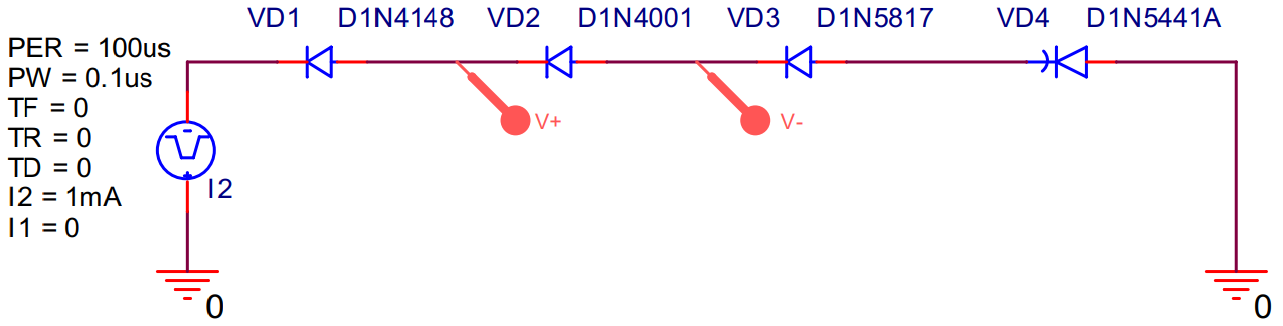
\includegraphics[width = 0.9 \textwidth]{scheme_1}
	\caption{\footnotesize Схема моделирования заряда барьерной емкости}
	\label{scheme_1}
	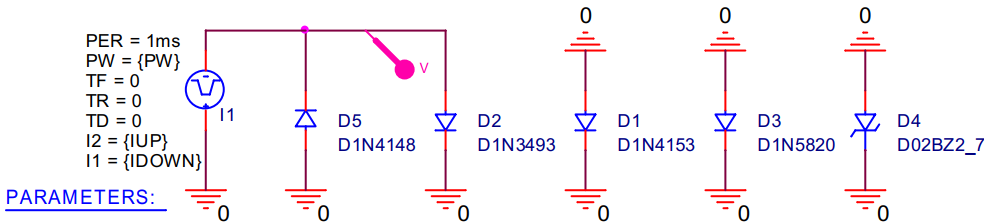
\includegraphics[width = 0.9 \textwidth]{scheme_3}
	\caption{\footnotesize Схема моделирования процесса рассасывания неосновных носителей}
	\label{scheme_3}
\end{figure}

\subsection*{2.1. Барьерная ёмкость}

\subsubsection*{Заряд барьерной ёмкости}

\textbf{{\normalsize 2.1.1.}}
Соединим диоды (кроме стабилитрона) по схеме, изображенной на рис. \ref{scheme_1}.\\
Установим параметры импульса: исходное состояние I1 = 0, амплитуда импульса
I2~=~1uA~-~10mA (зависит от диода), задержка TD = 0, длительность фронта TR~=~0, длительность спада TF = 0, длительность вершины импульса PW~=~10us, период повторения PER = 100us.\\
Для каждого диода подоберем I2 и Run to Time так, чтобы обратное напряжение к концу интервала наблюдения достигало 10V - 50V, но не превышало напряжения пробоя (Bv в модели).
Амплитуда тока I2 должна быть много больше максимального обратного тока диода.

\vspace{2cm}

\begin{figure}[H]
	\centering
	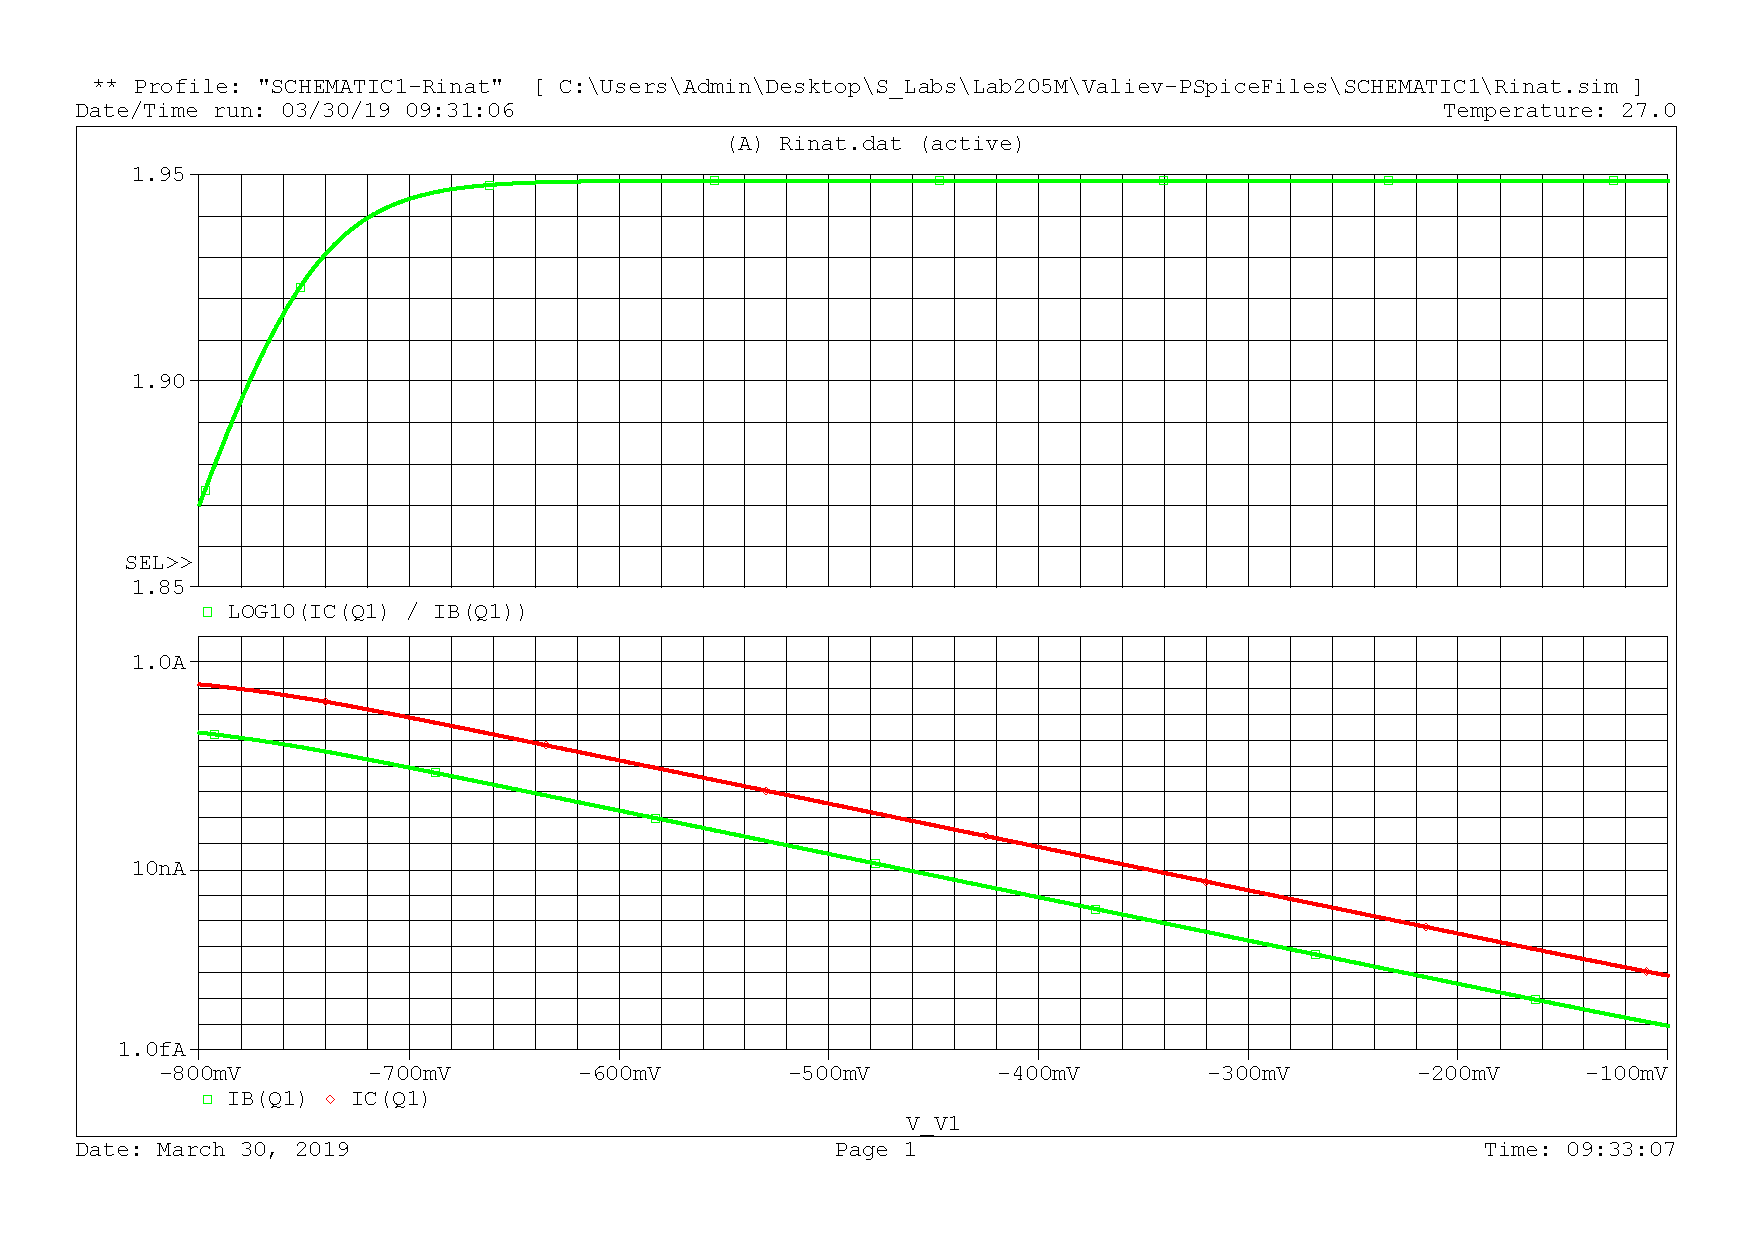
\includegraphics[width = 1 \textwidth]{1-1}
	\caption{D1N4149}
\end{figure}

\begin{figure}[H]
	\centering
	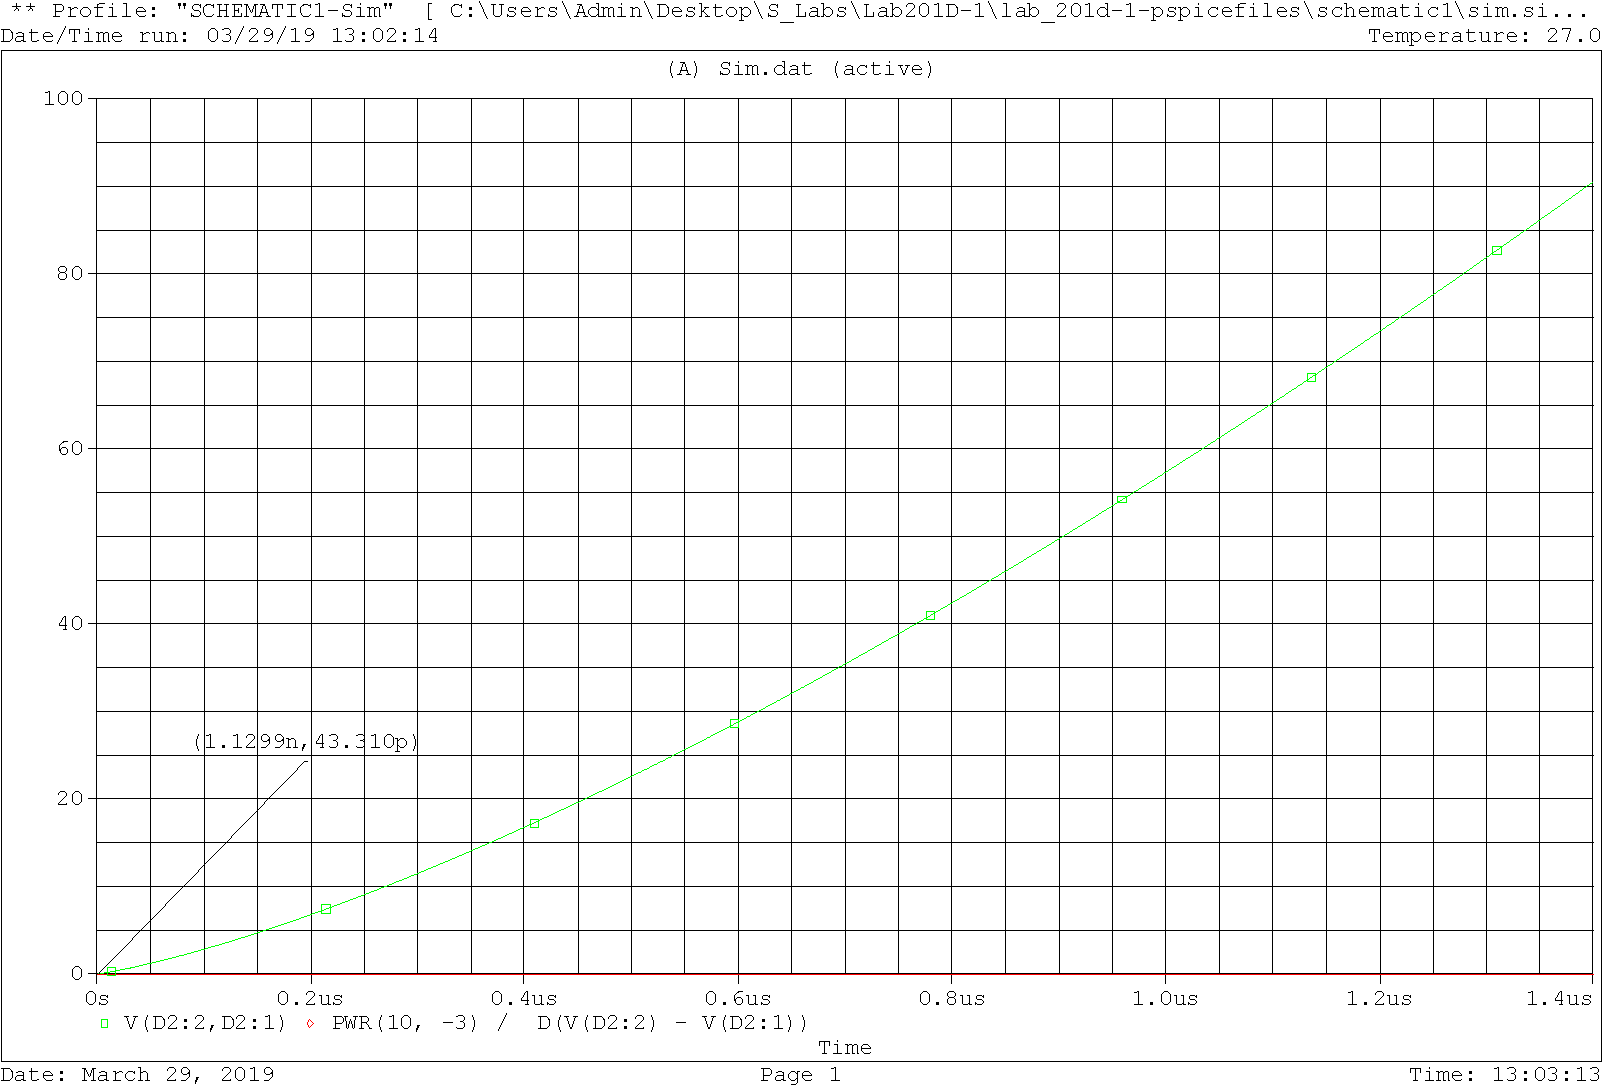
\includegraphics[width = 1 \textwidth]{1-2}
	\caption{D1N4002}
\end{figure}

\begin{figure}[H]
	\centering
	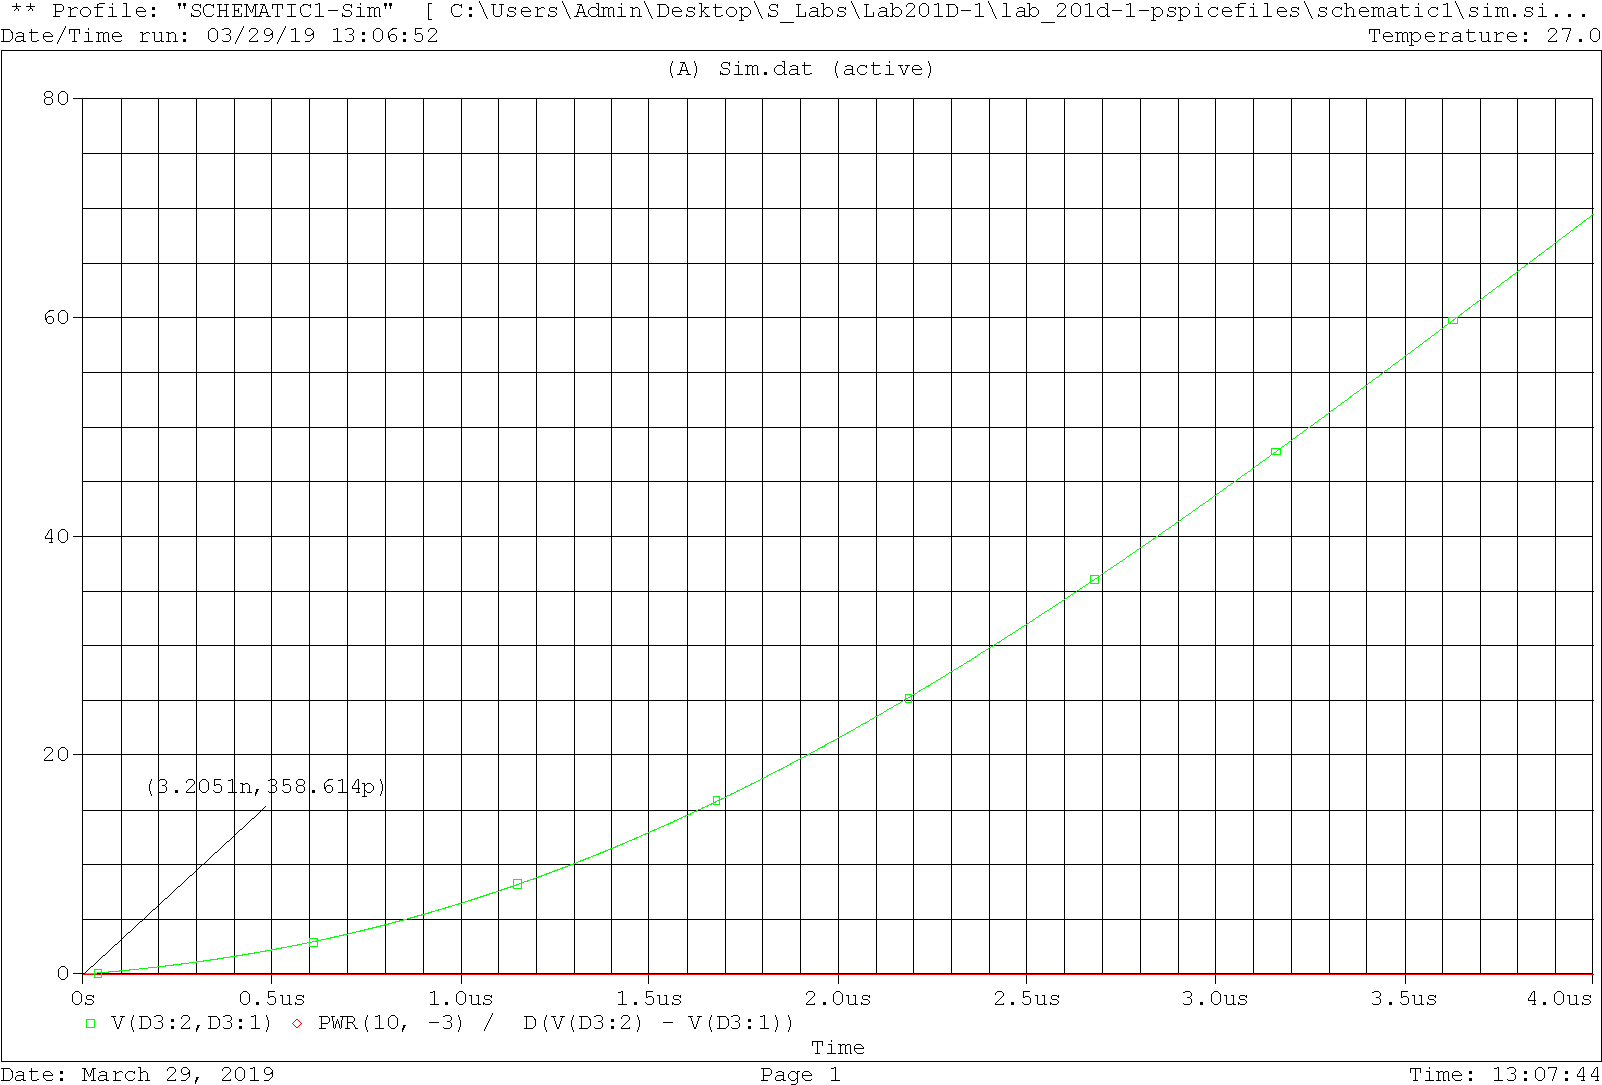
\includegraphics[width = 1 \textwidth]{1-3}
	\caption{D1N5818}
\end{figure}

\begin{figure}[H]
	\centering
	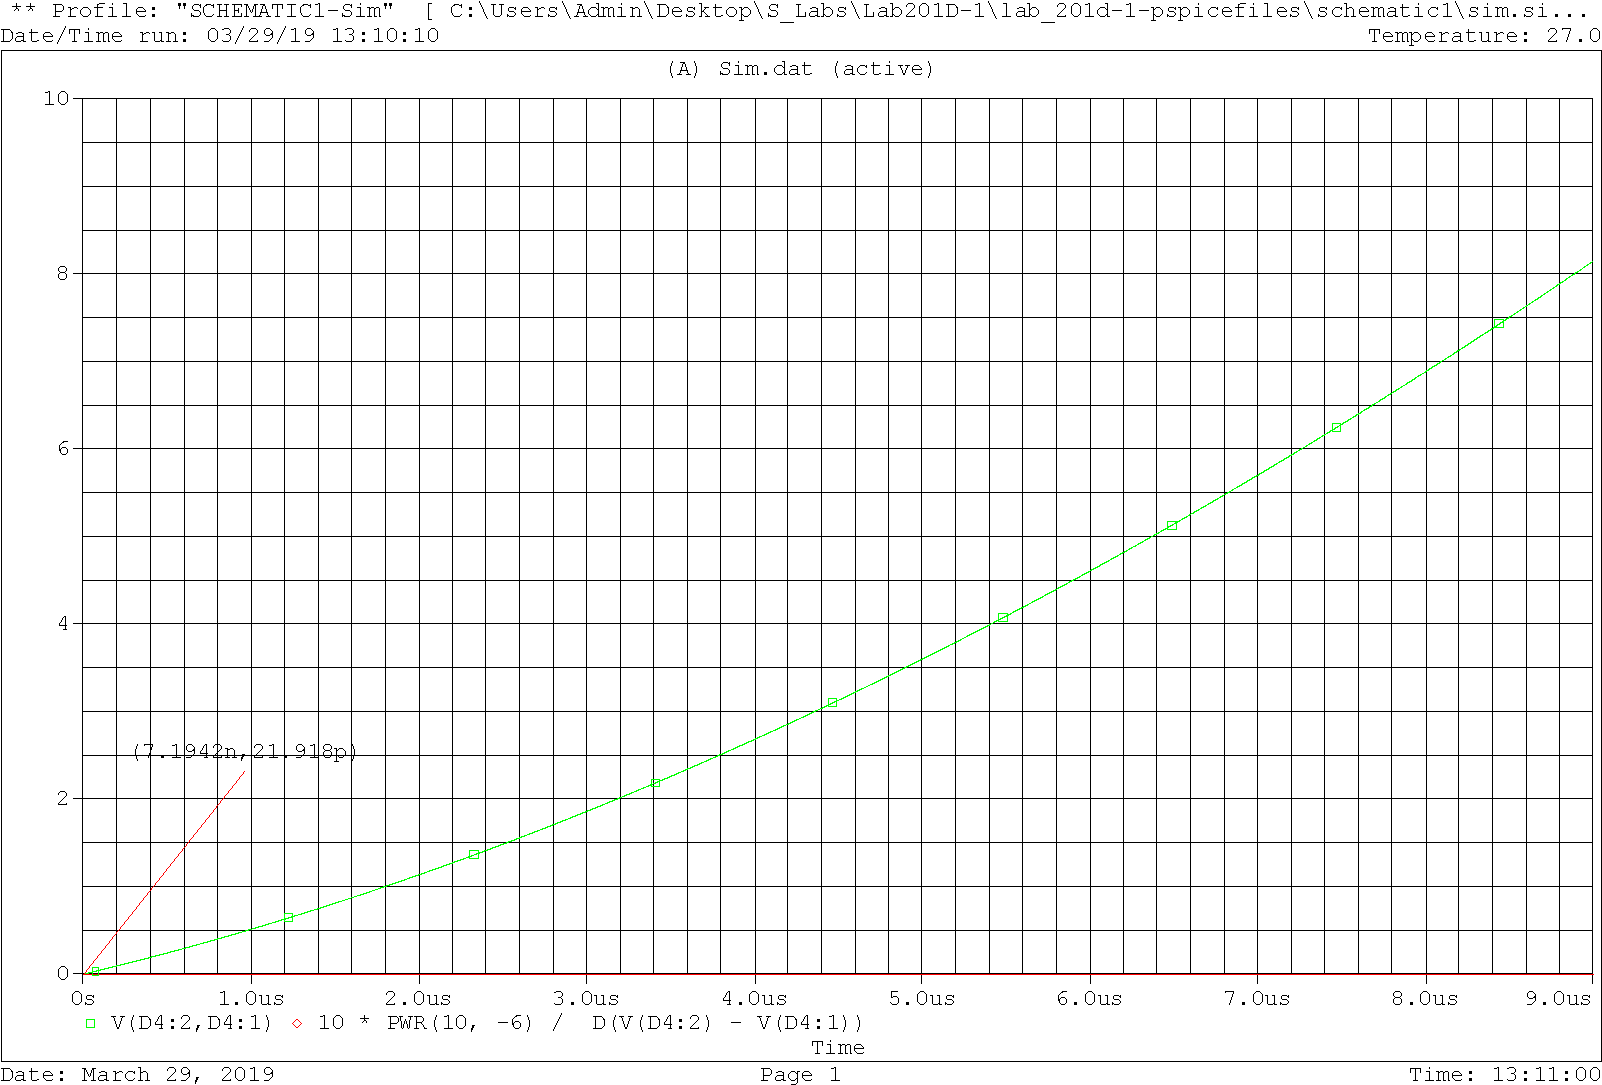
\includegraphics[width = 1 \textwidth]{1-4}
	\caption{D1N5443A}
\end{figure}


\textbf{{\normalsize 2.1.1.а.}}
Из временных диаграмм каждого диода определим производную и рассчитаем величину барьерной ёмкости $ C_{j0} $ при нулевом напряжении на диоде:

\begin{equation}
	C_{j0}\approx \left(I_2 \middle/  \frac{\Delta U}{\Delta t}\right)
\end{equation}

Сравним результаты со значениями $C_{j0}$ модели.

Значения барьерных ёмкостей были получены с помощью рассчетного блока \textbf{OrCAD} и приведено на графиках, изображённых выше.

\begin{table}[H]
	\centering
	\begin{tabular}{|c|c|c|c|c|}
		\hline
		&D1N4149 &D1N4002 &D1N5818 &D1N5443A \\ \hline 
		Эксп. $C_{j0}$ & 2p & 43p & 359p & 22p \\ \hline
		Теор. $C_{j0}$ & 2p & 51p & 359p & 22p \\ \hline
	\end{tabular}
	\caption{Сравнение значений барьерных емкостей}
	\label{tab_diodes}
\end{table}

\subsubsection*{Зависимость барьерной ёмкости от напряжения и температуры}

\begin{wrapfigure}{r}{5cm}
	\vspace{-0.7cm}
	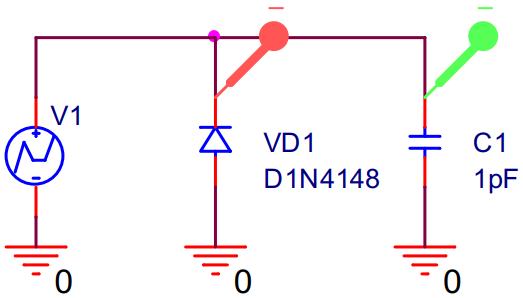
\includegraphics[width=5cm]{scheme_2}
	\caption{Схема соединения}
	\label{scheme_2}
\end{wrapfigure}

\textbf{{\normalsize 2.1.2.}}
Для каждого диода составим схему моделирования зависимости барьерной емкости от “обратного” напряжения (рис. \ref{scheme_2}).
Получим зависимости токов от времени. По известной крутизне и емкости конденсатора определим масштаб напряжения (горизонтальной оси) и масштаб емкости (вертикальной оси).

\begin{figure}[H]
	\centering
	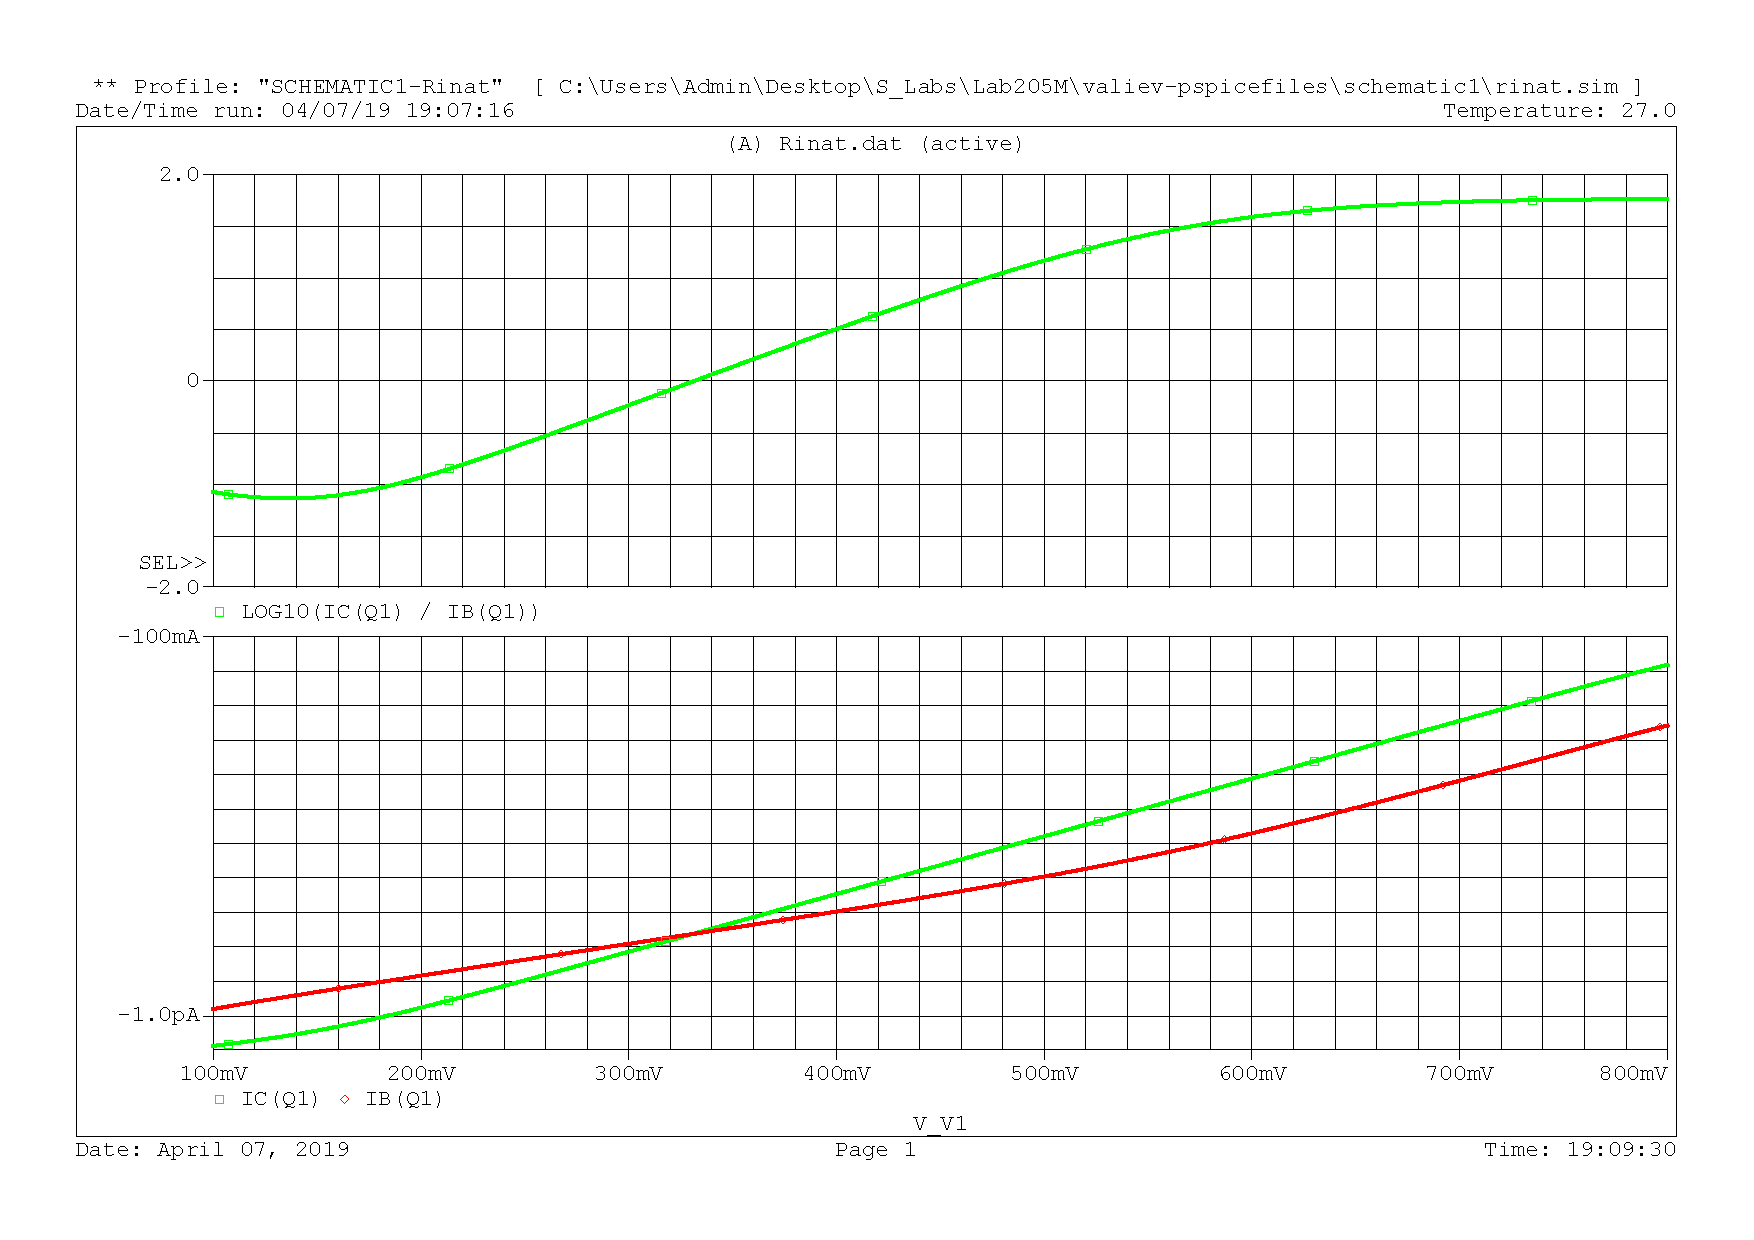
\includegraphics[width = 1 \textwidth]{2-1}
	\caption{D1N4149}
\end{figure}

\begin{figure}[H]
	\centering
	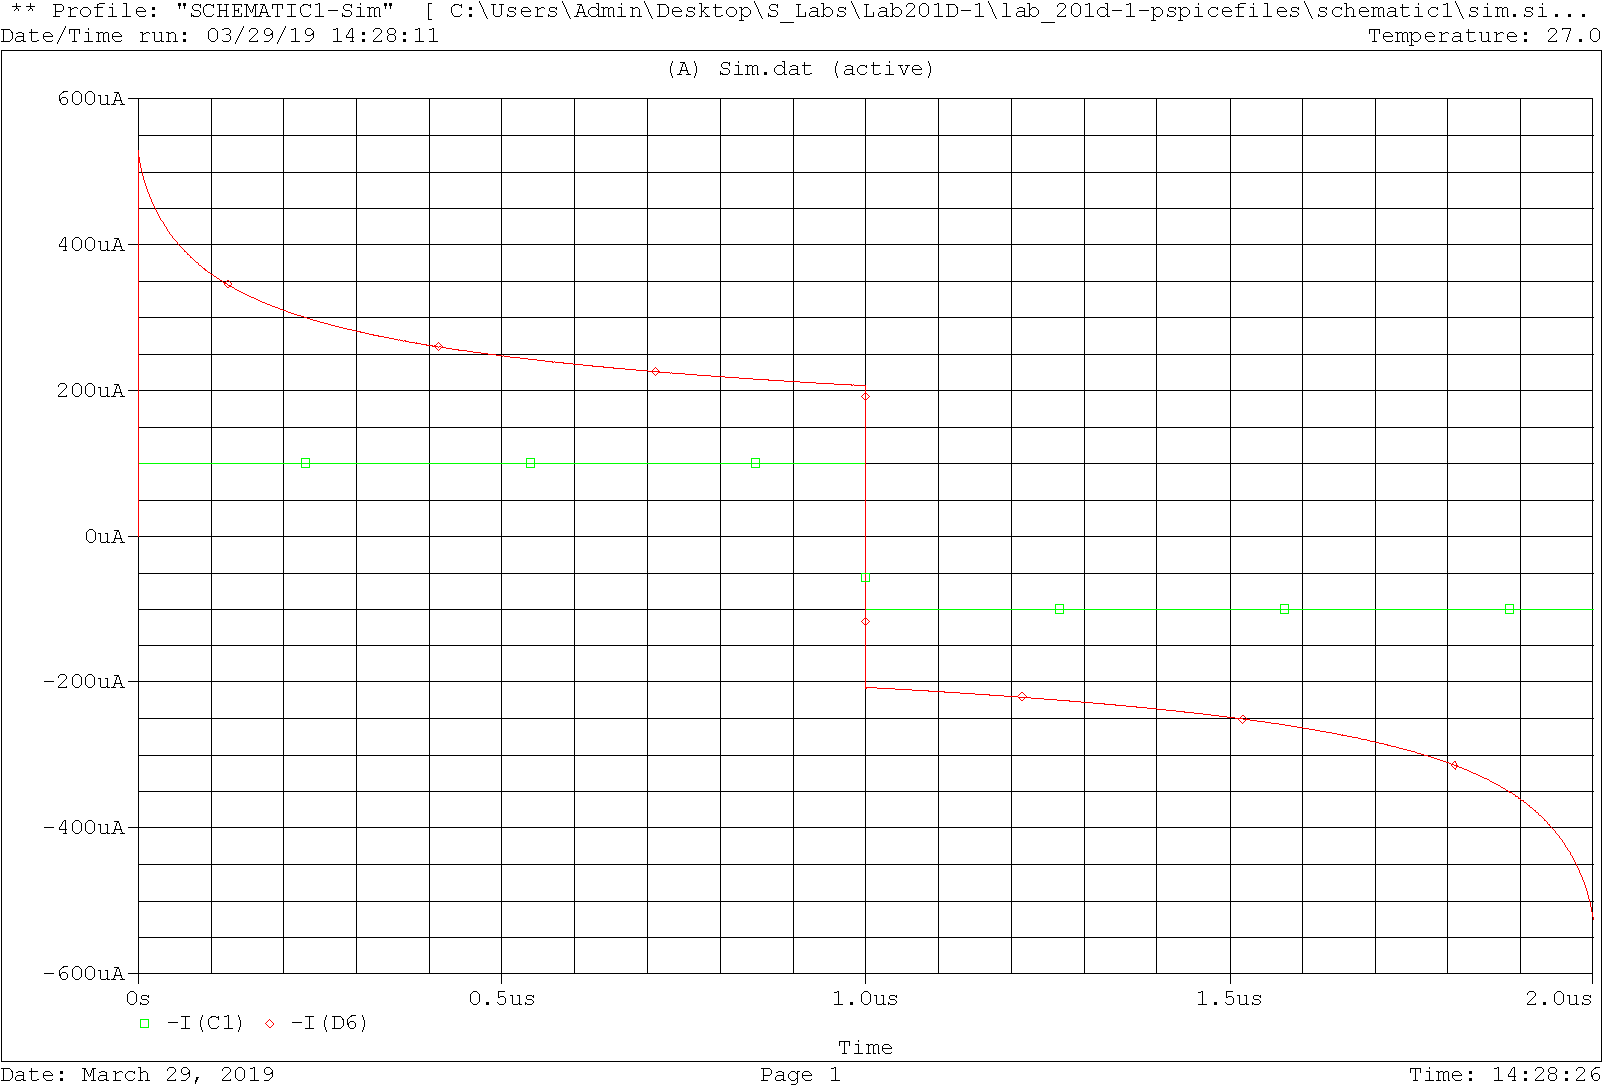
\includegraphics[width = 1 \textwidth]{2-2}
	\caption{D1N4002}
\end{figure}

\begin{figure}[H]
	\centering
	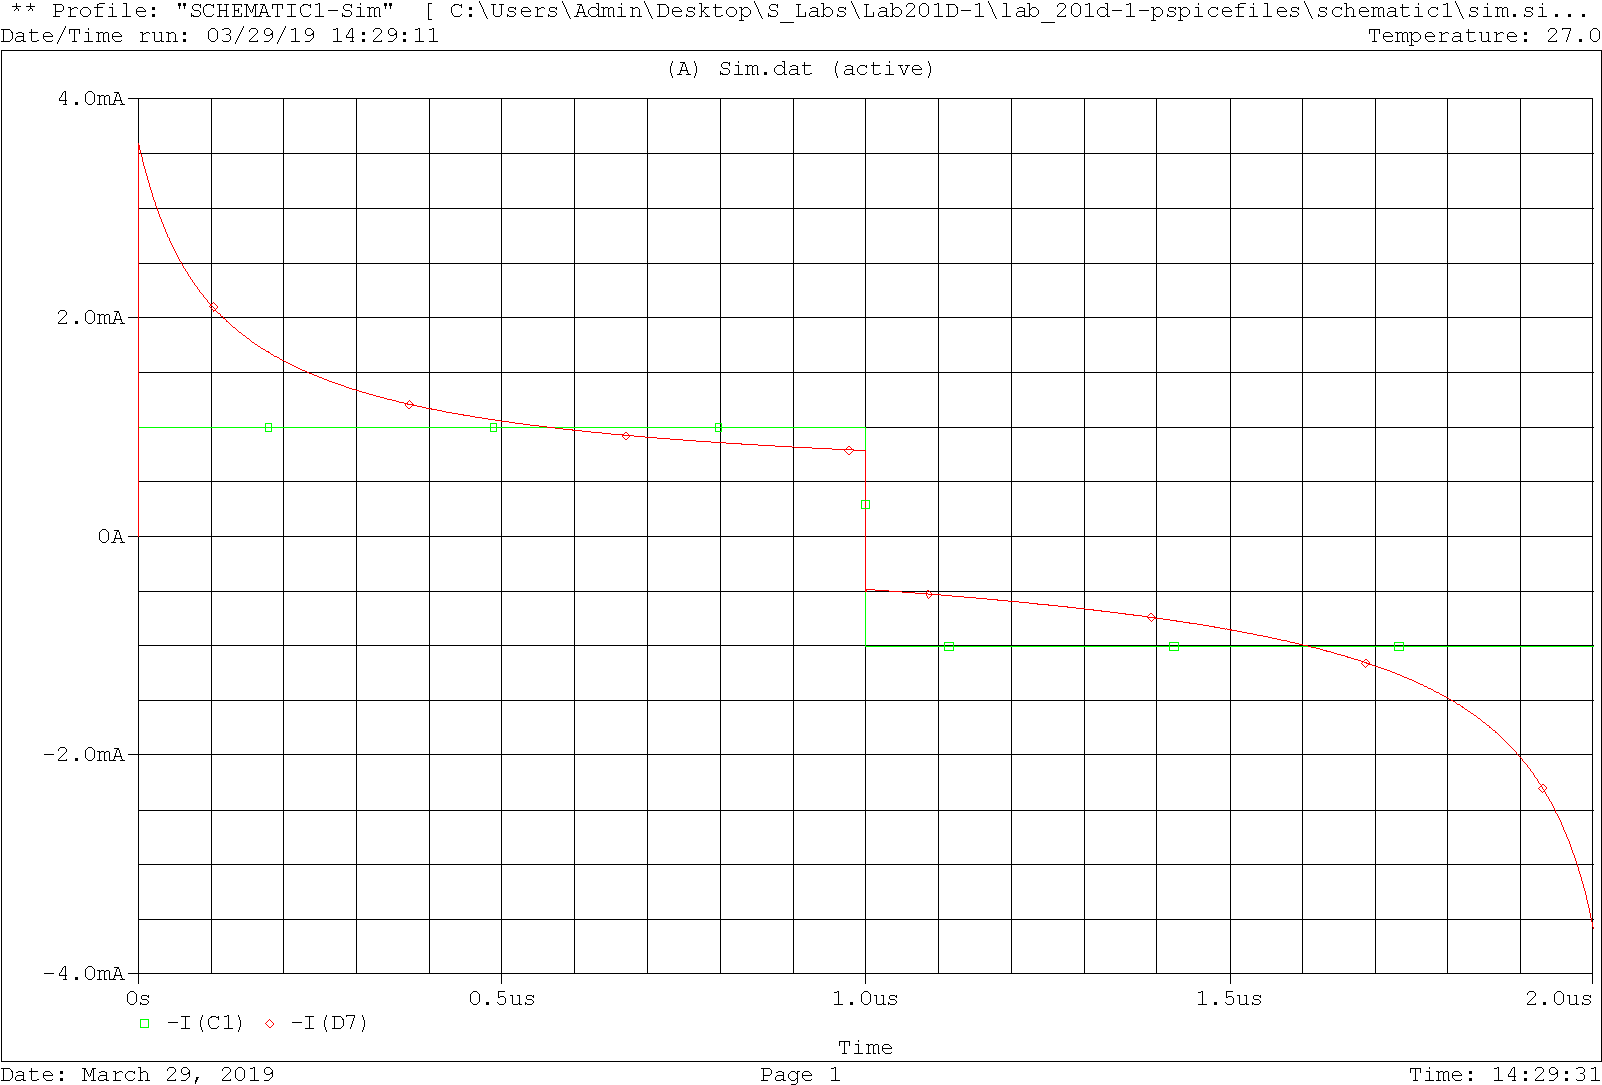
\includegraphics[width = 1 \textwidth]{2-3}
	\caption{D1N5818}
\end{figure}

\begin{figure}[H]
	\centering
	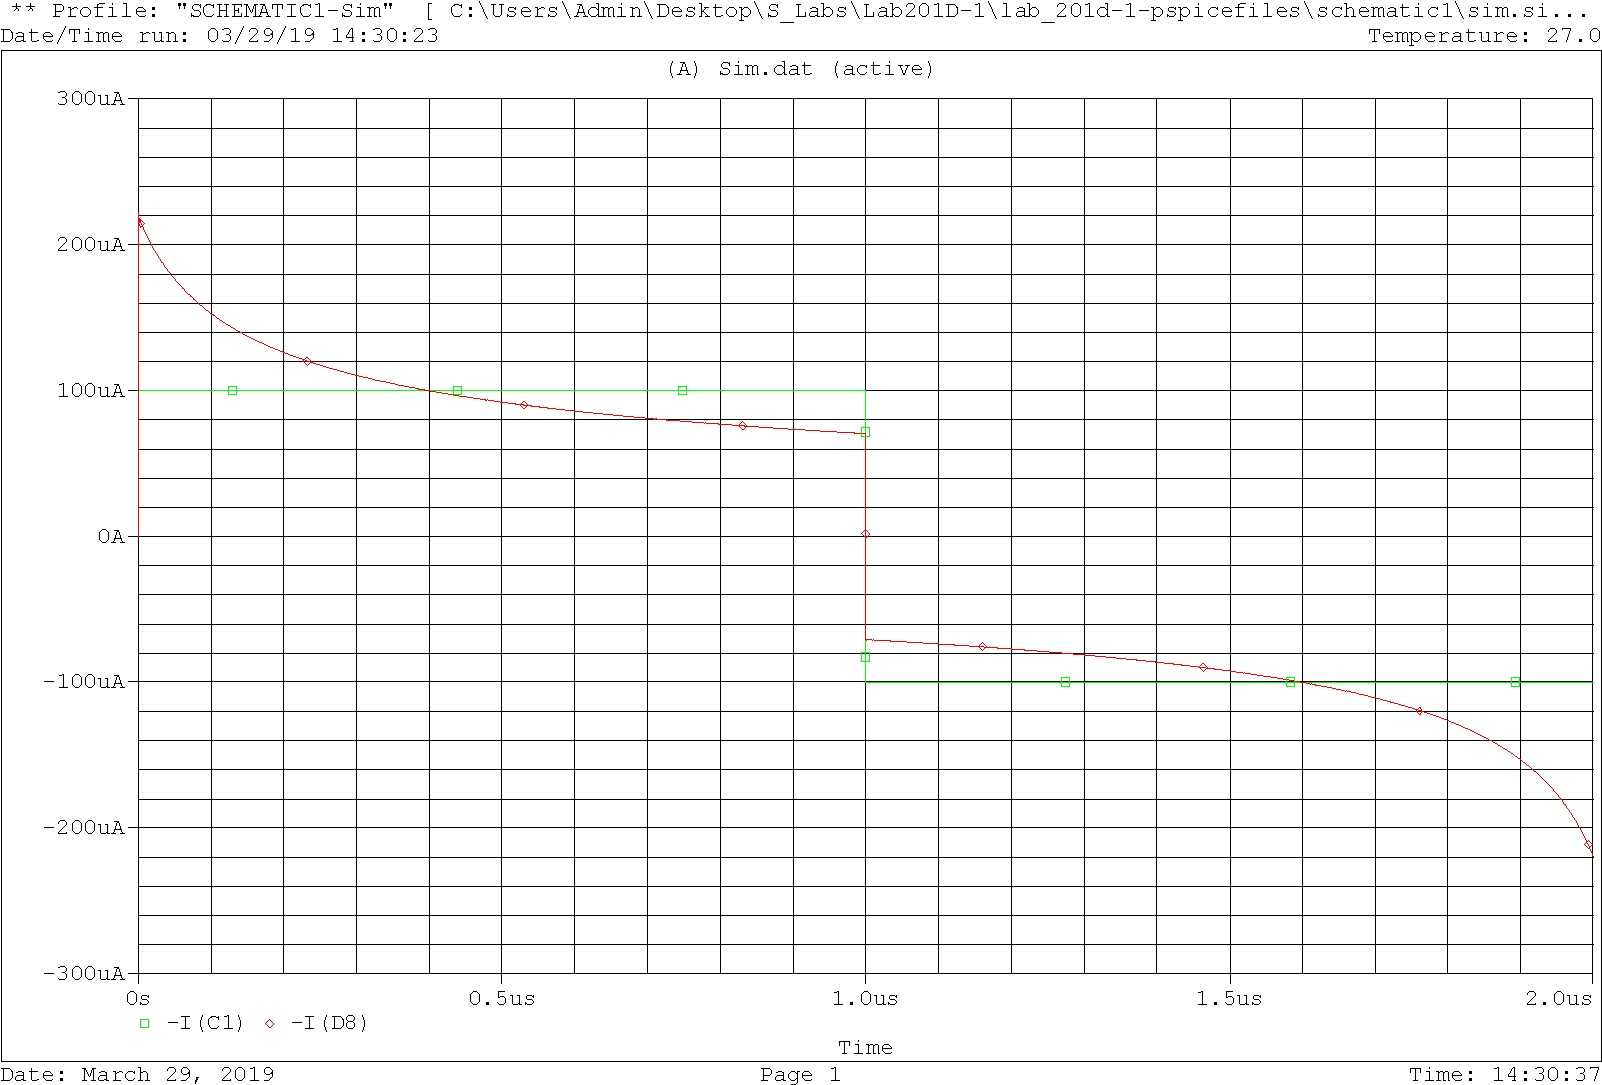
\includegraphics[width = 1 \textwidth]{2-4}
	\caption{D1N5443A}
\end{figure}

\begin{figure}[H]
	\centering
	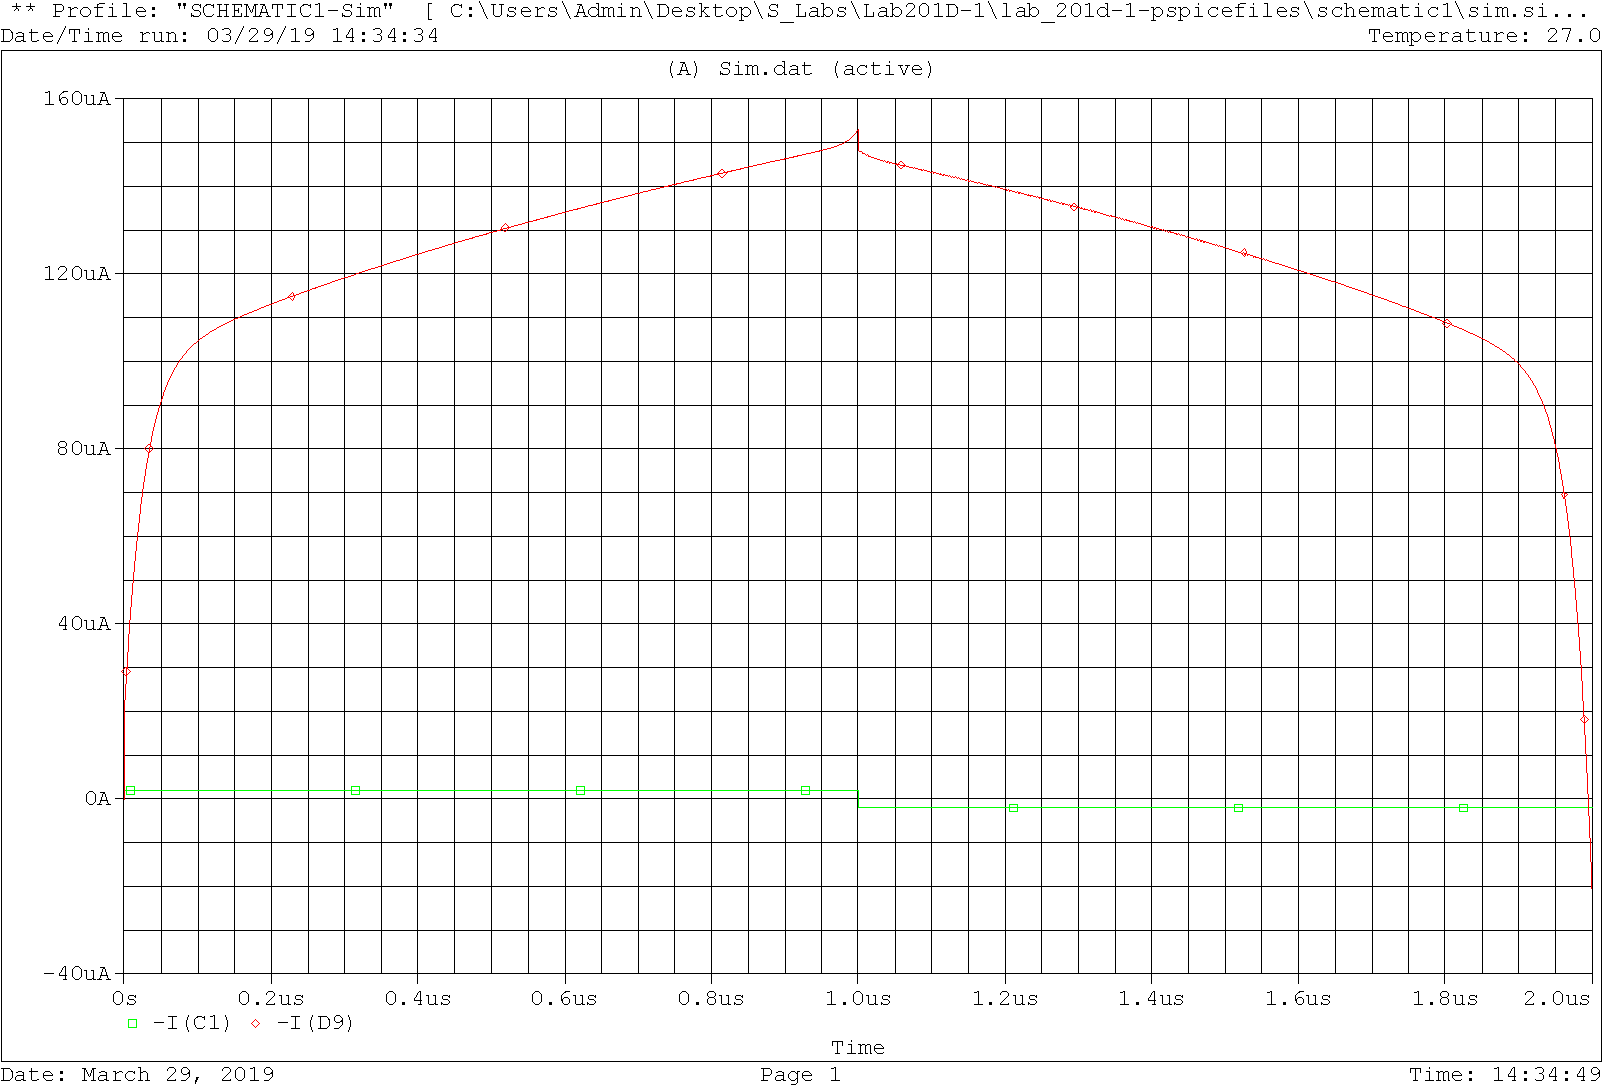
\includegraphics[width = 0.95 \textwidth]{2-5}
	\caption{D04AZ2\_2}
\end{figure}

%\newpage

\textbf{{\normalsize 2.1.2.a.}}
Для импульсного ВЧ диода дополнительно для –60, 27,120 градусов Цельсия получим семейство температурных зависимостей барьерной ёмкости.

\begin{figure}[H]
	\centering
	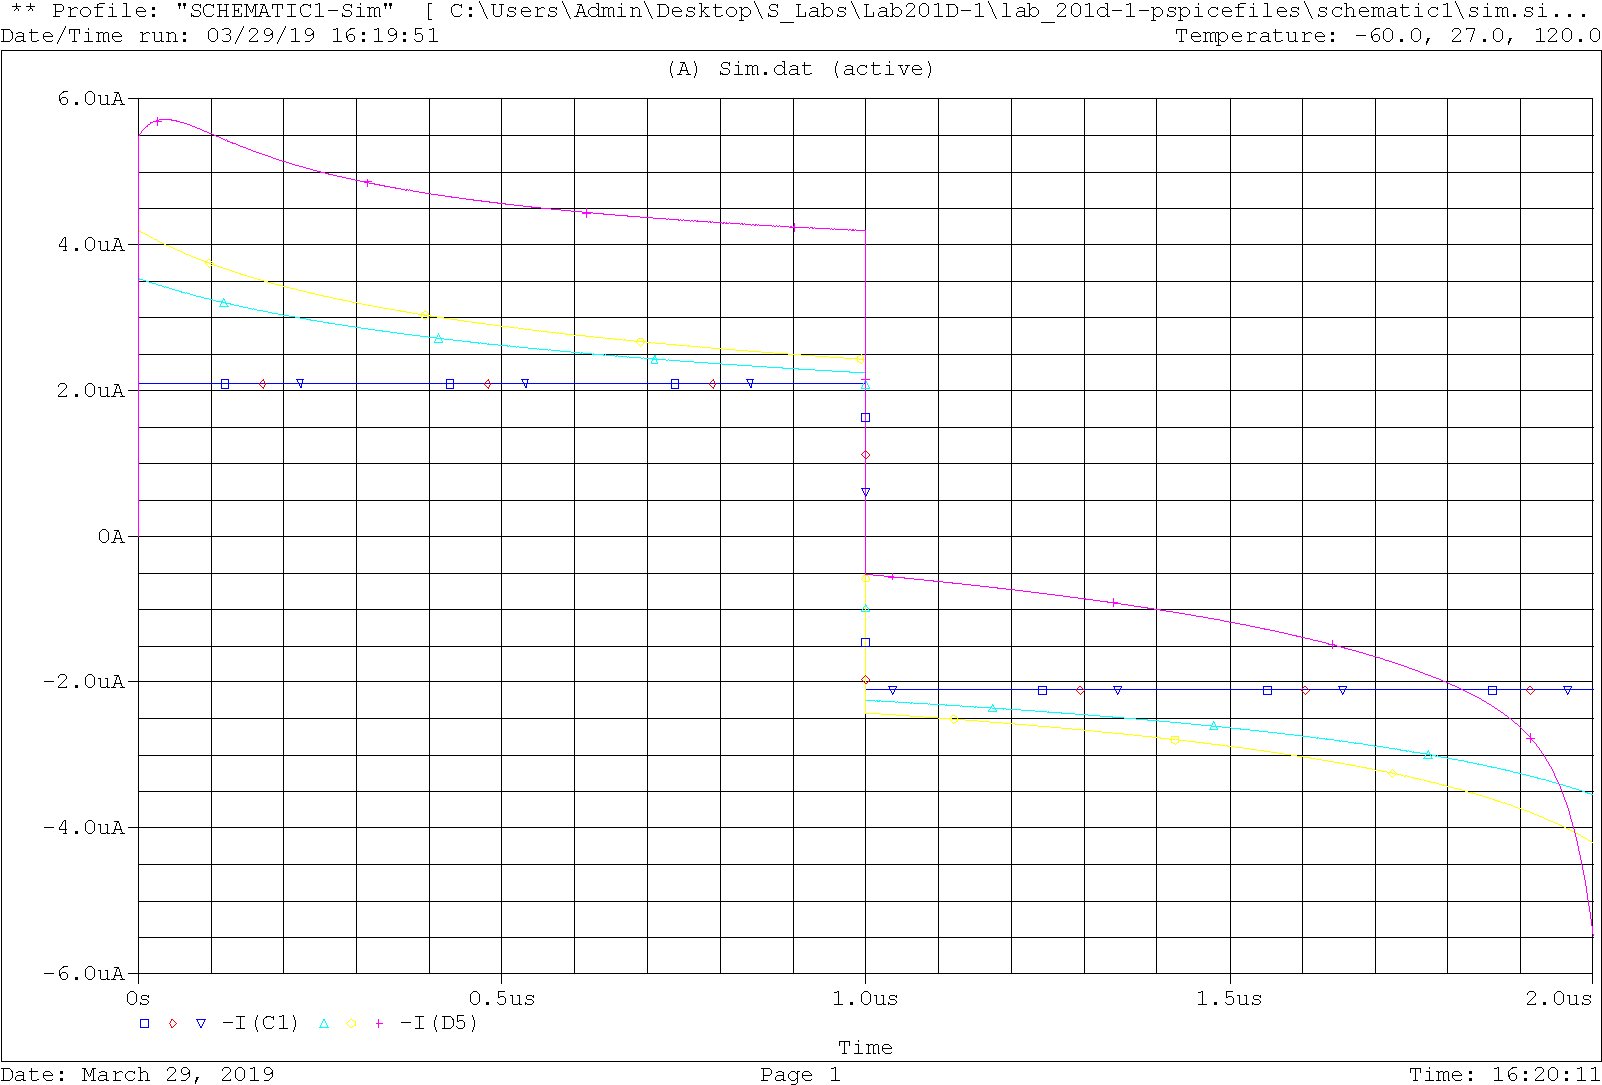
\includegraphics[width = 0.95 \textwidth]{3}
	\caption{D1N4149}
\end{figure}

\begin{center}
	\[T=-60 \Cd: ~~~ C_{бар}=1.8pF\]
	\[T= 27 \Cd: ~~~ C_{бар}=2pF\]
	\[T=120 \Cd: ~~~ C_{бар}=2.39pF\]
\end{center}

\textbf{{\normalsize 2.1.2.б.}}
Проверим соответствуют ли полученные в пункте 2.1.2 зависимости барьерных емкостей диодов от напряжения теоретической зависимости. Определим $ U_0 $.\\

\begin{center}
	D1N4149:  $U_0 = 1.67 V$ \\
	D1N4002:  $U_0 = 2.11 V$ \\	
	D1N5818:  $U_0 = 2.53 V$ \\
	D1N5443A: $U_0 = 2.12 V$ \\
	Для стабилитрона приближение не выполняется.
\end{center}

\textbf{{\normalsize 2.1.2.в.}}
Предложим метод получения зависимости барьерной емкости от обратного напряжения при сравнимых токах $C \cdot dU/dt$ и $I_{sr}$.\\

При выбранных масштабах крутизны и емкости можно будет построить сдвоенную систему координат, затем из-за линейности импульсов источника можно будет определить величину барьерной ёмкости через ёмкость нормировочного конденсатора.\\

\textbf{{\normalsize 2.1.2.г.}}
Как зависит оценка (по результатам моделирования) $C_{j0}$ от обратного тока диода?

Линейным образом в области нормировки дополнительным конденсатором согласно устройству источника.

\newpage

\subsubsection*{2.2 Диффузионная ёмкость}

\textbf{{\normalsize 2.2.1.}}
Импульсами тока этого генератора накапливаются неосновные носители (“заряжается диффузионная емкость”) исследуемого диода, а в паузе между импульсами рассасываются не основные носители (“диффузионная емкость разряжается”). Время разряда диффузионной емкости определяется по задержке начала разряда барьерной емкости после спада импульса I1.\\
Проведем временное моделирование для напряжения на диоде. Для каждого диода
подоберем параметры PW импульсов, Run Time и Maximum step size.\\

\begin{figure}[H]
	\centering
	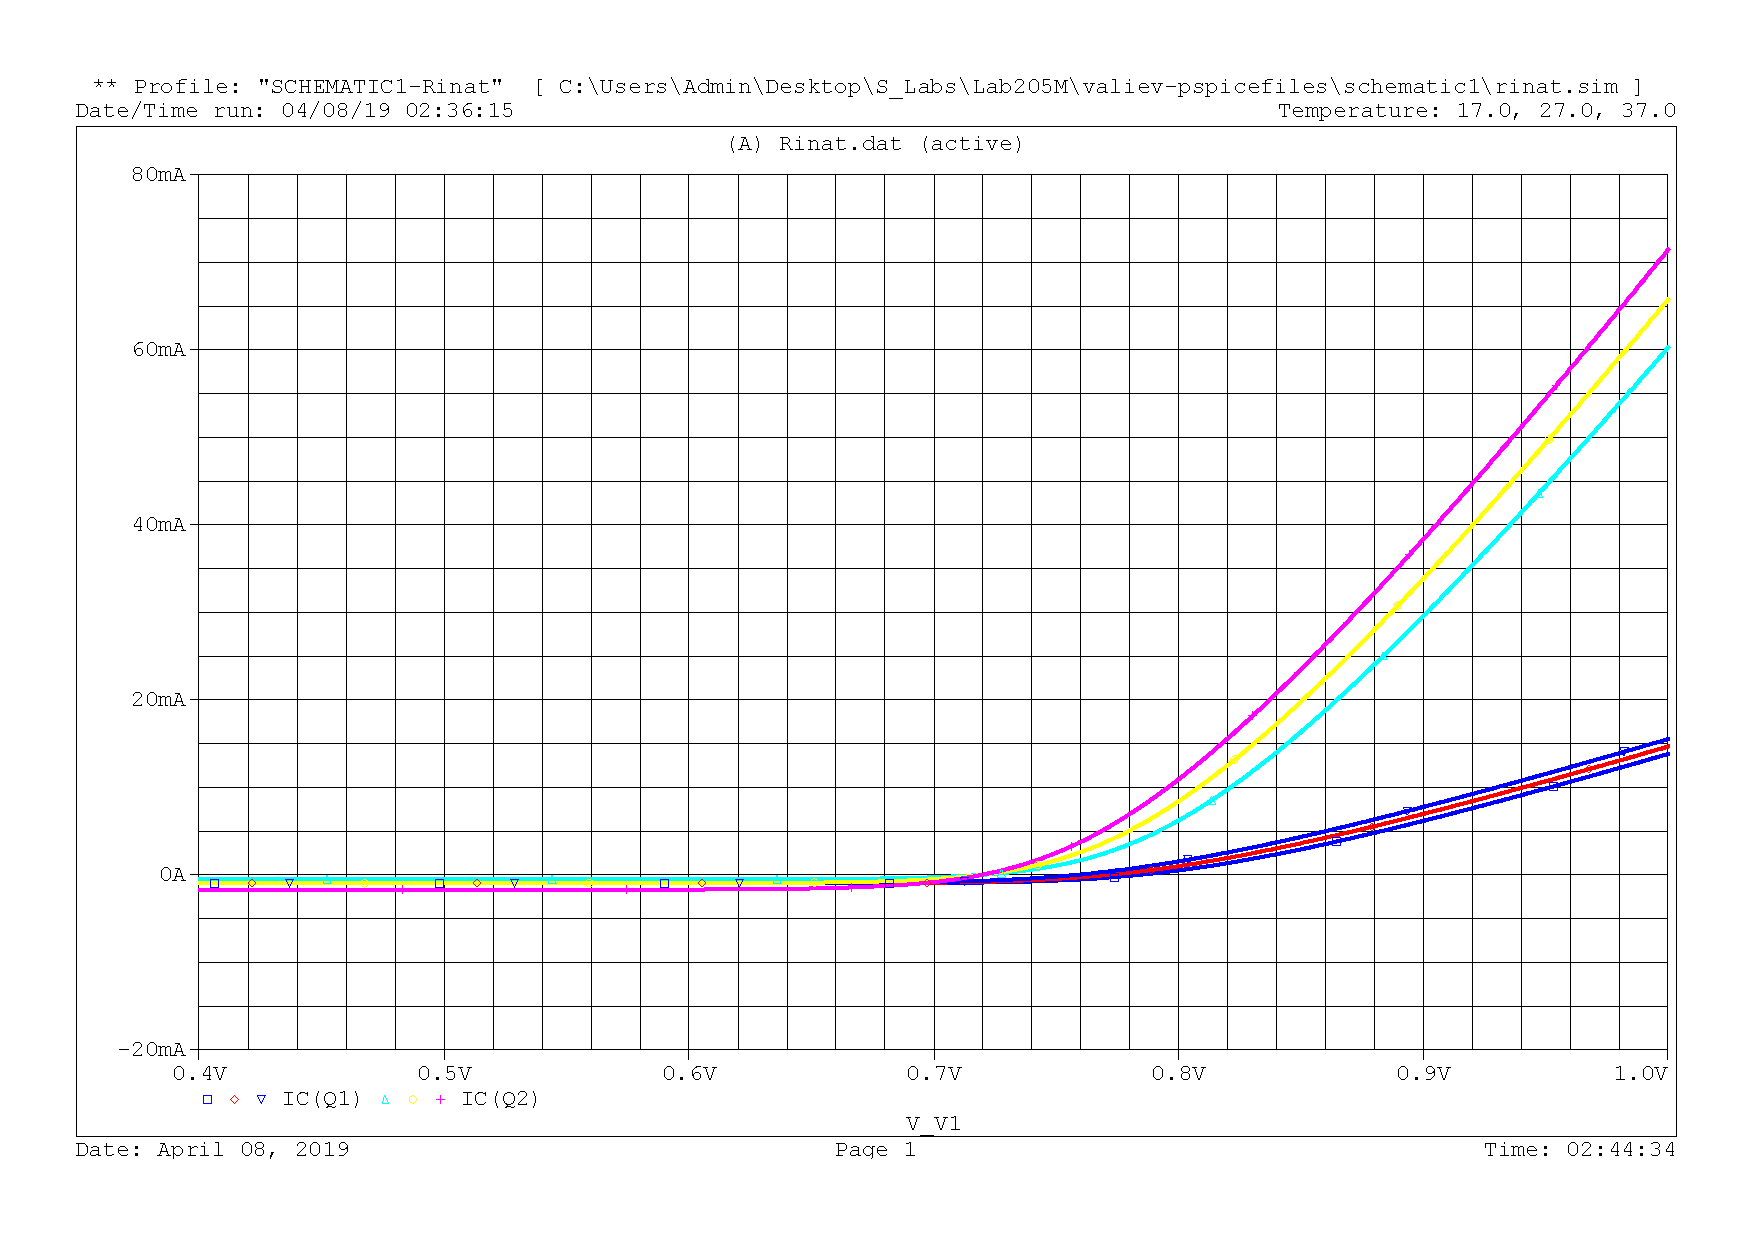
\includegraphics[width = 1 \textwidth]{4-1}
	\caption{D1N4149}
\end{figure}

\begin{figure}[H]
	\centering
	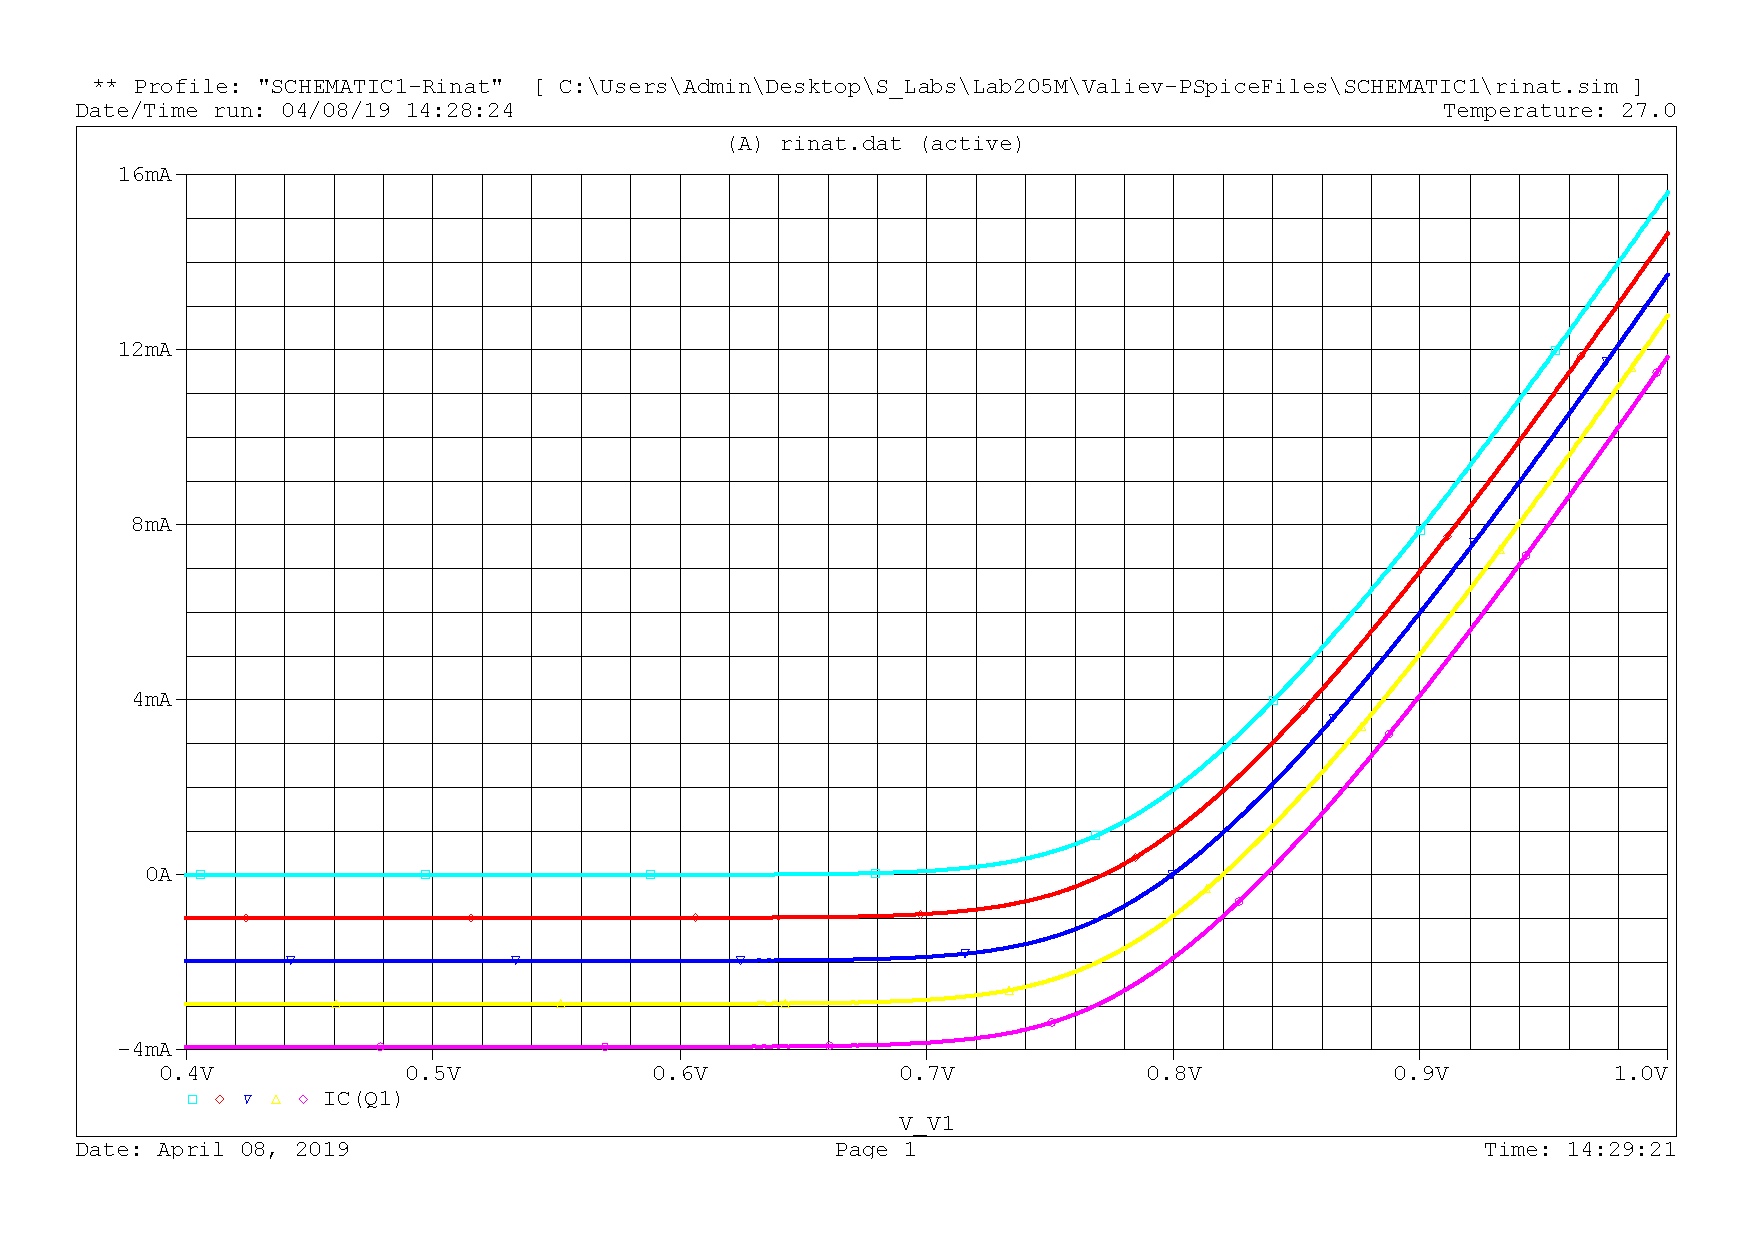
\includegraphics[width = 1 \textwidth]{4-2}
	\caption{D1N4002}
\end{figure}

\begin{figure}[H]
	\centering
	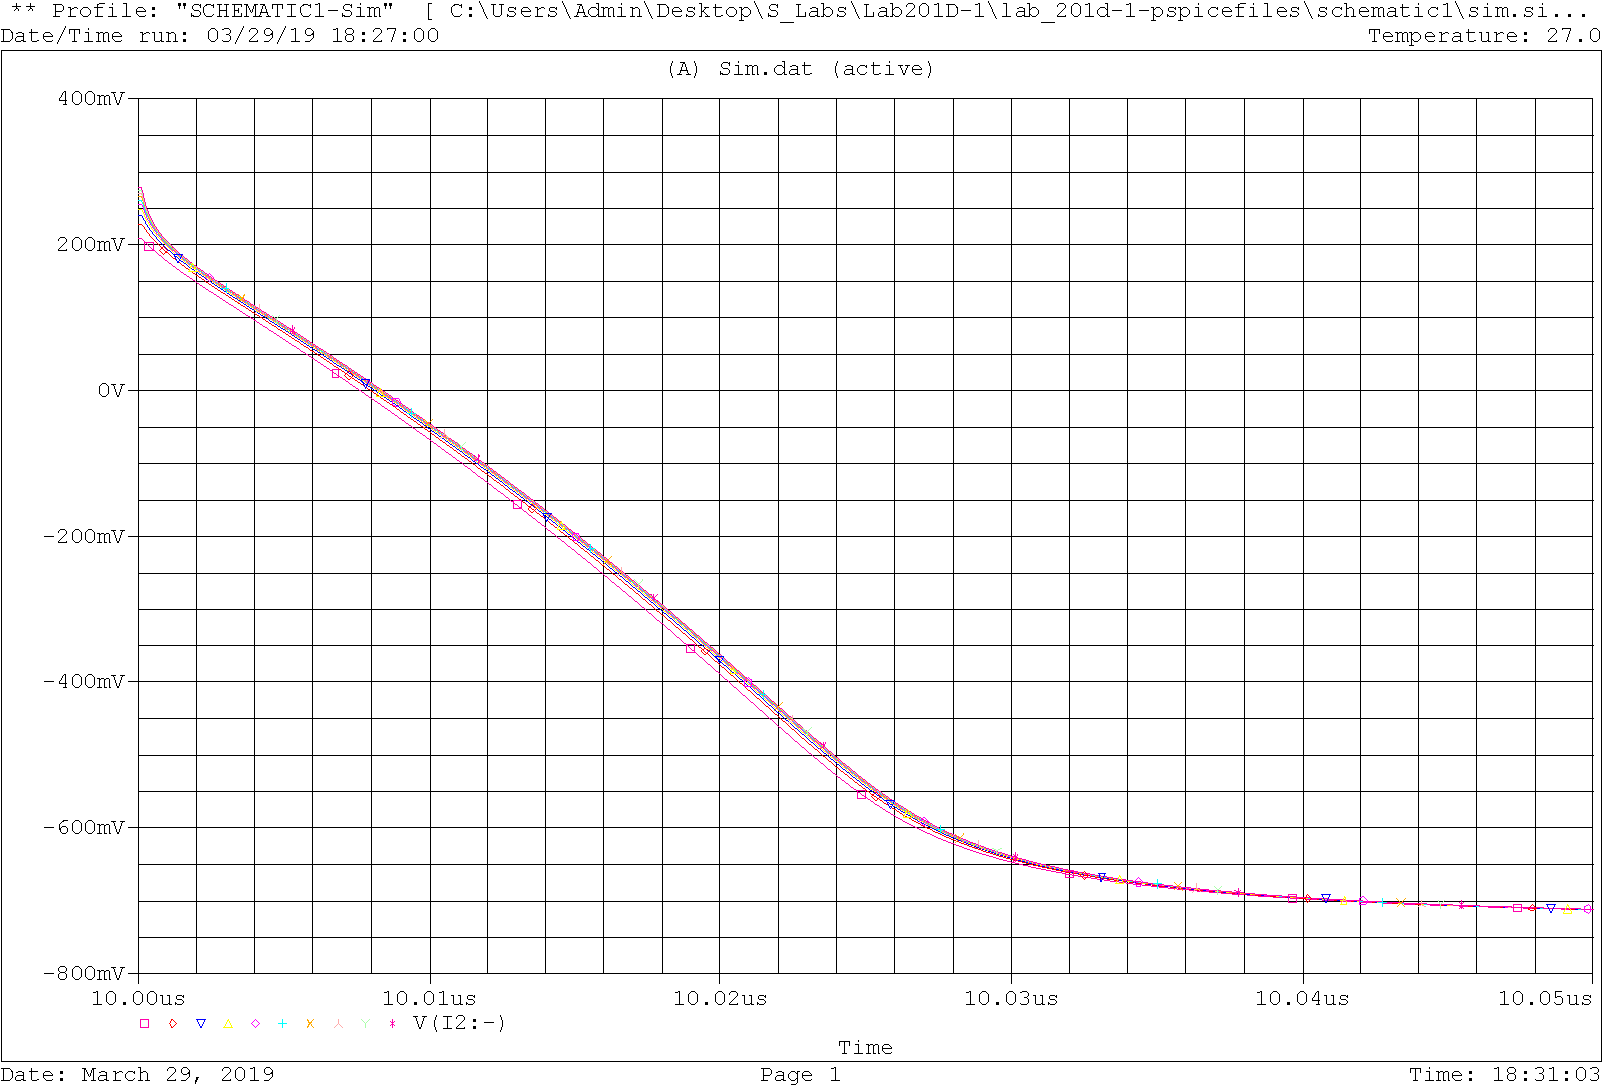
\includegraphics[width = 1 \textwidth]{4-3}
	\caption{D1N5818}
\end{figure}

\begin{figure}[H]
	\centering
	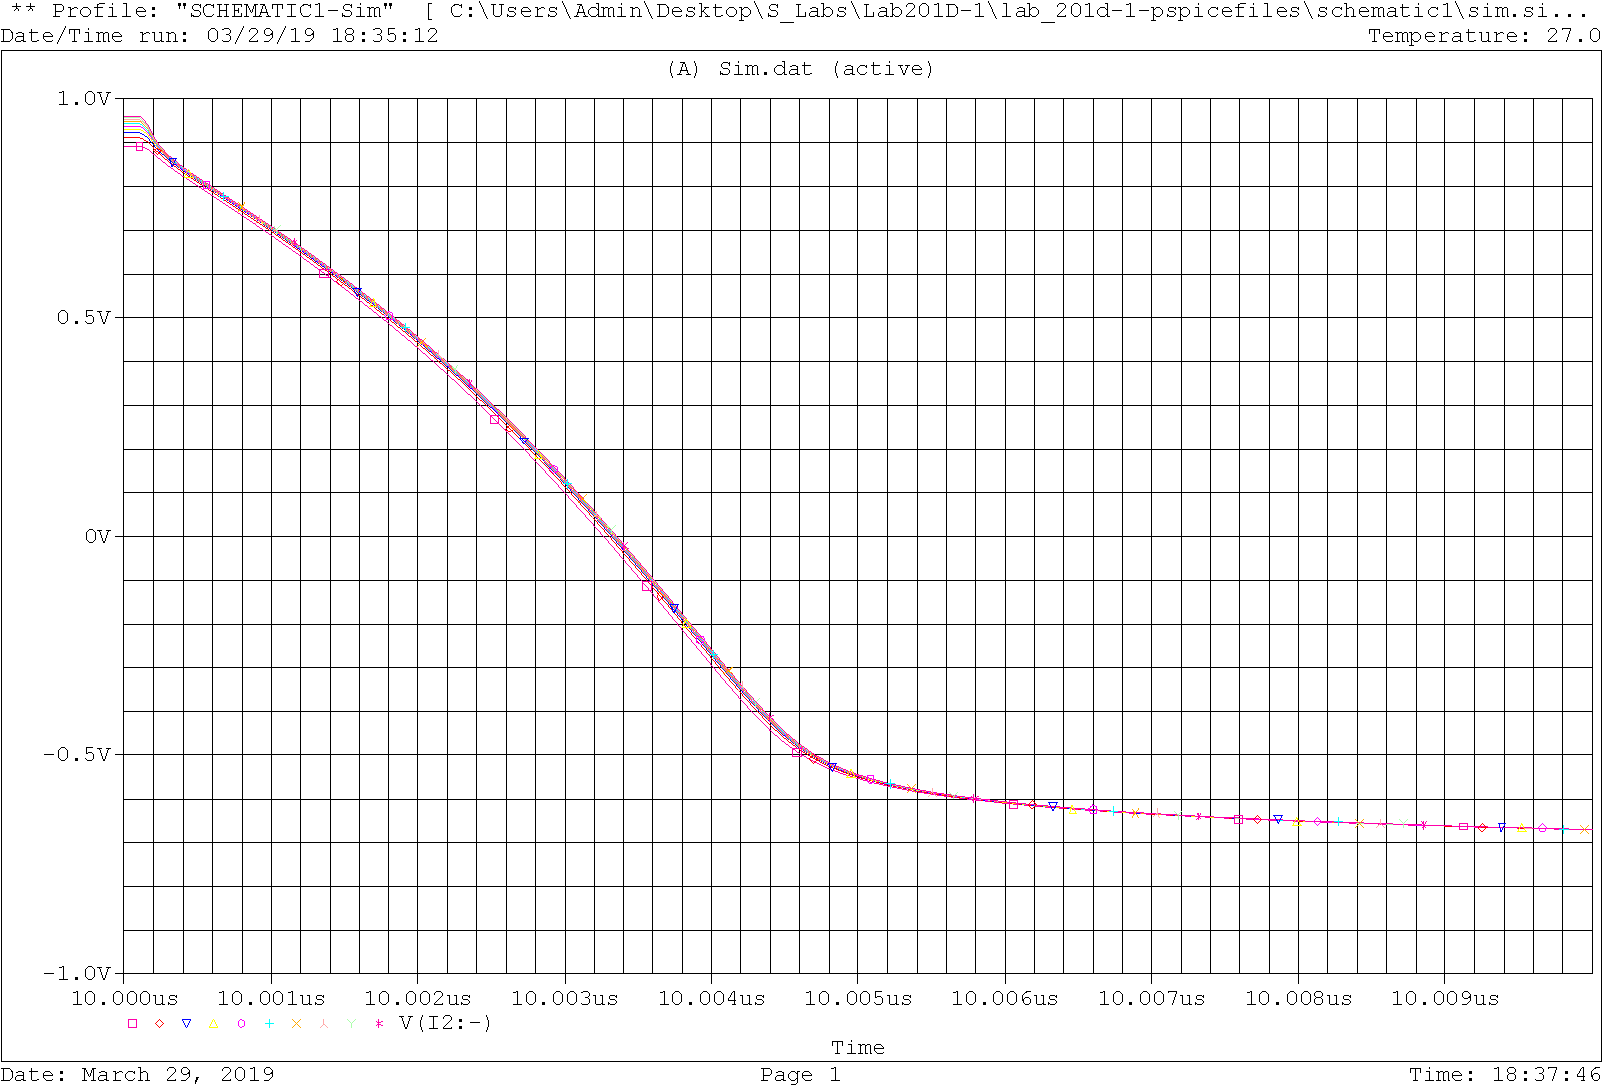
\includegraphics[width = 1 \textwidth]{4-4}
	\caption{D1N5443A}
\end{figure}

\begin{figure}[H]
	\centering
	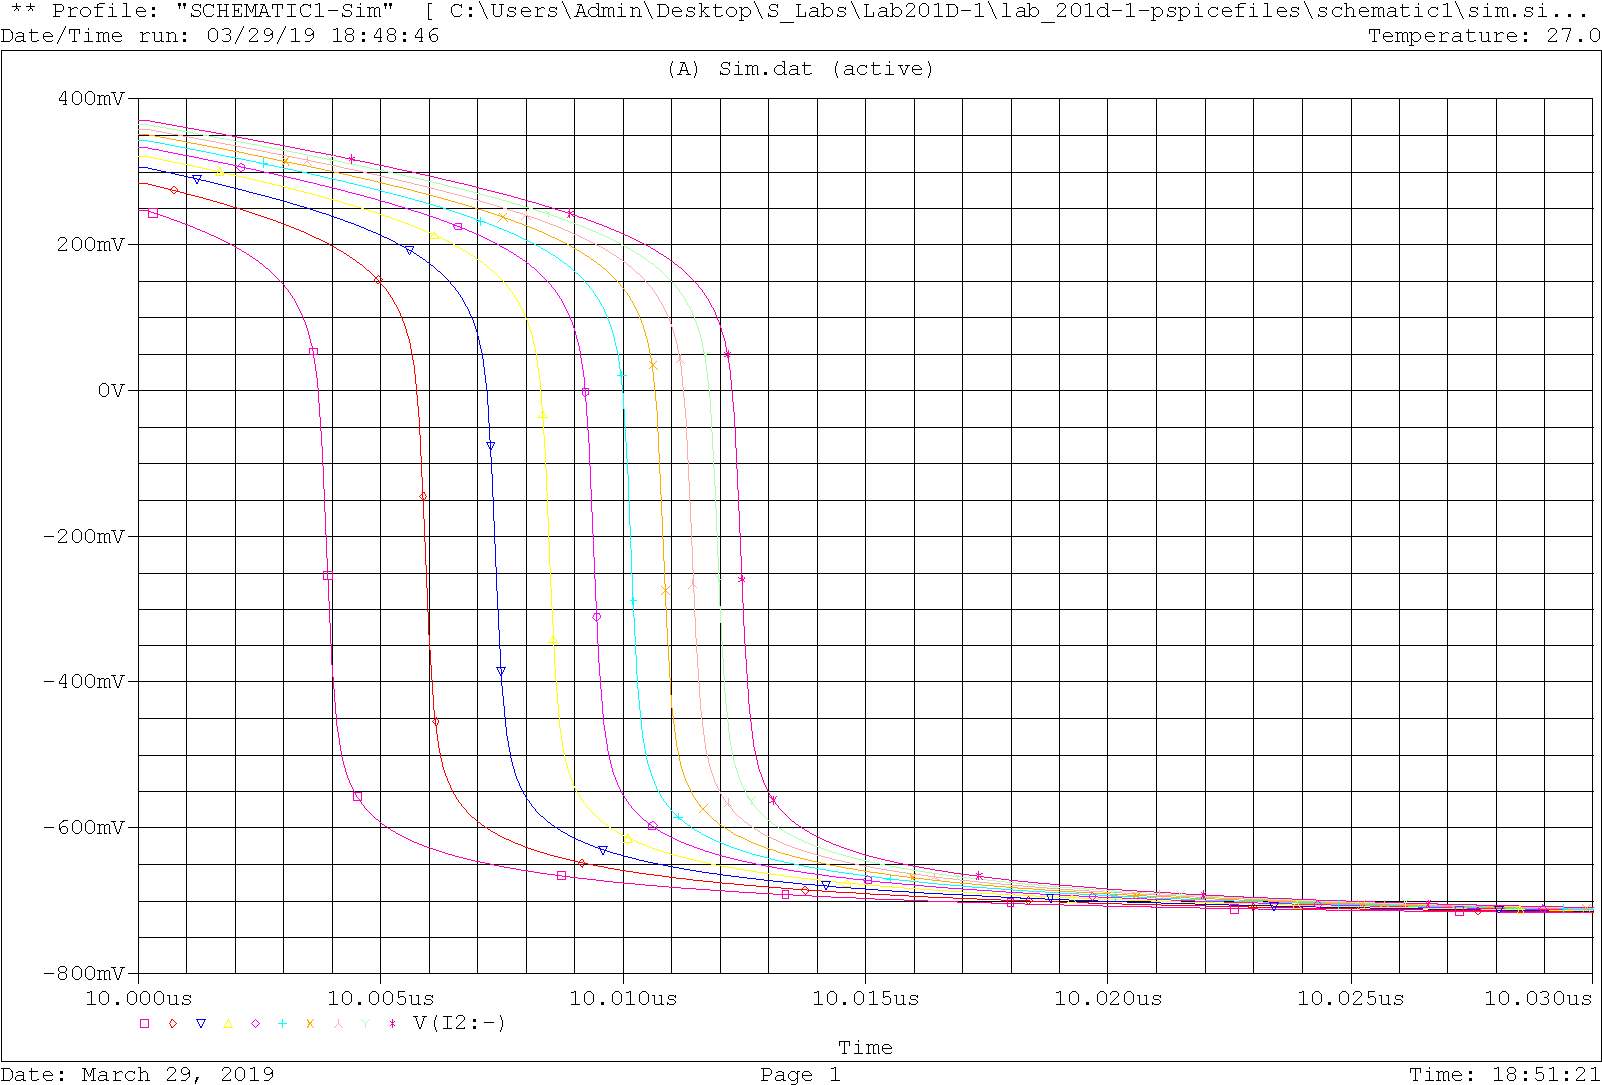
\includegraphics[width = 1 \textwidth]{4-5}
	\caption{D04AZ2\_2}
\end{figure}


\textbf{{\normalsize 2.2.1.a.}}
Для импульсного ВЧ диода по скачку напряжения рассчитаем сопротивление $R_s$. Сравним с паспортными данными модели.\\

\begin{center}
	\[R_s=\dfrac{\Delta U}{\Delta I} = \dfrac{0.872-0.816}{0.1} \Omega \approx 0.56 \Omega \]
	\[R_s^{табл} = 0.5664 \Omega \]
\end{center}
\textbf{{\normalsize 2.2.1.б.}}
Для импульсного ВЧ диода для I1 = 10mA и дискретных значений IUP = I2 = 17.21mA, 100mA напечатаем на графике время разряда диффузионной ёмкости. Рассчитаем время жизни ННЗ для I2 = 17.21mA и время разряда диффузионной ёмкости для I2 = 100mA.\\

\begin{figure}[H]
	\centering
	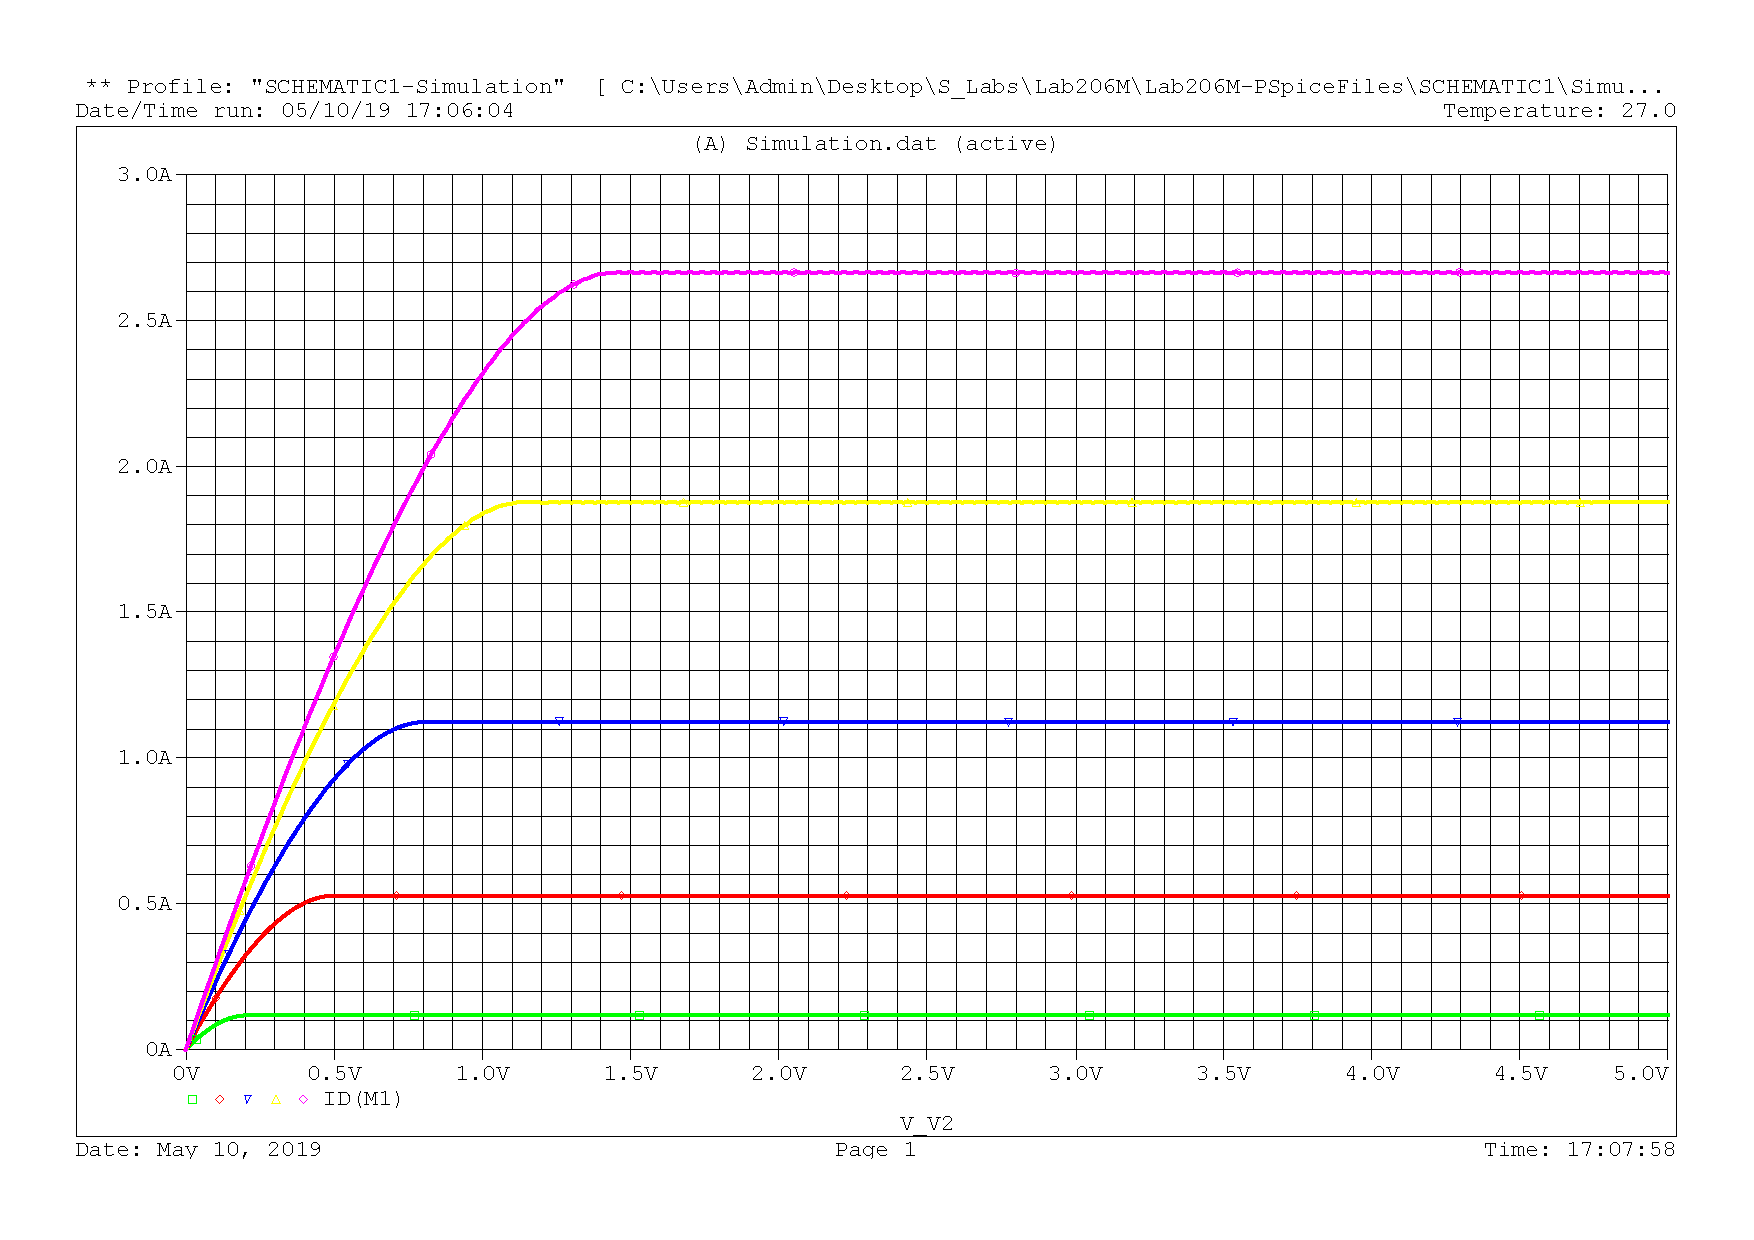
\includegraphics[width = 1 \textwidth]{5}
	\caption{D1N4149}
\end{figure}

\begin{center}
	\[ \tau_{рас} = 6 ns; \text{  } \tau_p = \dfrac{\tau_{рас}}{1+ln\left(\frac{I_2}{-I_1}\right)} = 3.7 ns\]
	\[ \tau_{pас} = 14 ns; \text{   } \tau_{рас} = \tau_{p}\cdot \left(1+ln\left(\frac{I_2}{-I_1}\right)\right) = 11.8 ns\] 
\end{center}

\textbf{{\normalsize 2.2.1.в.}}
Оценим по результатам моделирования пункта 2.2.1 заряд неосновных носителей выпрямительного диода при заданном токе.

\[Q=|I_1\cdot \tau_p| \approx 40 pC \text{ для каждого из токов } I_2\]


\textbf{{\normalsize 2.2.1.г.}}
Объясним различие графиков разряда ёмкостей диода Шоттки и обычных диодов.\\

В диодах Шоттки в качестве барьера Шоттки используется переход металл - полупроводник, в отличие от обычных диодов, где используется p-n-переход. Особенностью такого перехода является отсутствие накопления избыточного заряда в базе. Инерционные свойства такого диода связаны с зарядом в барьерной емкости. Переход металл-полупроводник обладает рядом особенных свойств (отличных от свойств полупроводникового p-n-перехода). К ним относятся: пониженное падение напряжения при прямом включении, высокий ток утечки, очень маленький заряд обратного восстановления. Последнее объясняется тем, что по сравнению с обычным p-n-переходом у таких диодов отсутствует диффузия, связанная с инжекцией неосновных носителей, т.е. они работают только на основных носителях, а их быстродействие определяется только барьерной ёмкостью.\\

Теоретически диод Шоттки может обладать низкой электрической ёмкостью барьера Шоттки. Отсутствие p-n-перехода позволяет повысить рабочую частоту.\\

\newpage

\textbf{{\normalsize 2.2.2.}}
Для выпрямительного диода получим аналогичные временные диаграммы напряжения для дискретных значений I1 = -10 mA, -50 mA, -100mA и I2 = 100mA = const.\\

\begin{figure}[H]
	\centering
	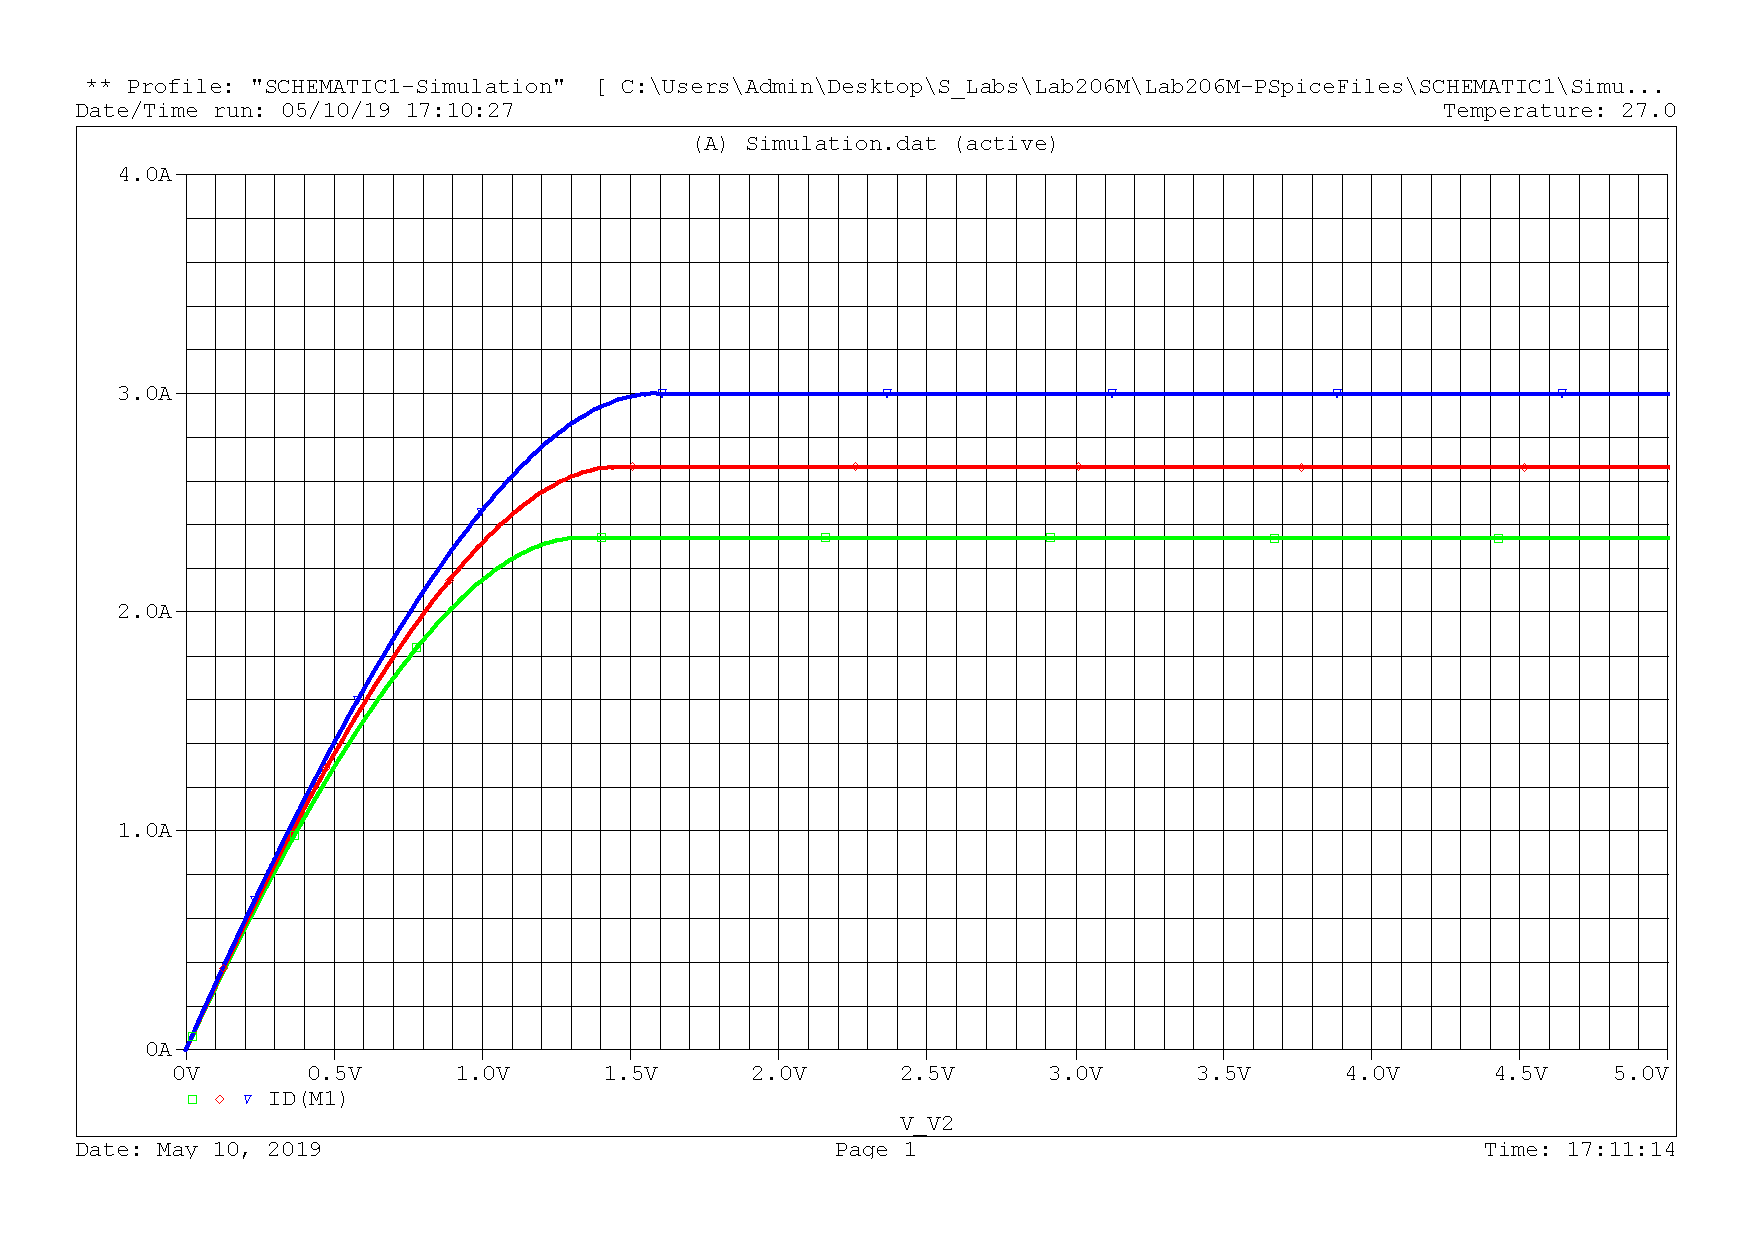
\includegraphics[width = 1 \textwidth]{6}
	\caption{D1N4002}
\end{figure}

\begin{center}
	\[ \tau_{рас} = 3.56 us; \text{  } \tau_p = \dfrac{\tau_{рас}}{1+ln\left(\frac{I_2}{-I_1}\right)} = 1.72 us\]
	\[ \tau_{рас} = 5.79 us; \text{   } \tau_p = \dfrac{\tau_{рас}}{1+ln\left(\frac{I_2}{-I_1}\right)} = 3.36 us\] 
	\[ \tau_{рас} = 13.37 us; \text{   } \tau_p = \dfrac{\tau_{рас}}{1+ln\left(\frac{I_2}{-I_1}\right)} = 5.78 us\] 
\end{center}

\end{document}